% =====================================================================
%  Designing Data Visualizations for Non-Expert Audiences
%  Phase 4 Final Research Paper -- IEEE conference format (IEEEtran)
% =====================================================================
\documentclass[conference]{IEEEtran}

\IEEEoverridecommandlockouts

% ---------- Packages ----------
\usepackage[utf8]{inputenc}
\usepackage[T1]{fontenc}
\usepackage{cite}
\usepackage{graphicx}
\usepackage{amsmath,amssymb,amsfonts}
\usepackage{mathtools}
\usepackage{textcomp}
\usepackage{xcolor}
\usepackage{booktabs}
\usepackage{array}
\usepackage{tabularx}
\usepackage{multirow}
\usepackage{enumitem}
\usepackage[hidelinks]{hyperref}

\setlist{nosep,leftmargin=*,itemsep=2pt,topsep=2pt}

% ---------- Convenience & Verified Dataset Macros ----------
\newcommand{\Tnorm}{T_{\mathrm{norm}}}
\newcommand{\Cnorm}{C_{\mathrm{norm}}}
\newcommand{\TCE}{\mathrm{TCE}}
\newcommand{\SCB}{\mathrm{SCB}}
\newcommand{\ADR}{\mathrm{ADR}}
\newcommand{\BS}{\mathrm{BS}}
\newcommand{\etap}{\eta_p^{2}}
\newcommand{\pp}{\,\text{pp}}
\newcommand{\Ctwo}{\textbf{C2}}
\newcommand{\Cone}{\textbf{C1}}
\newcommand{\Cthree}{\textbf{C3}}
\newcolumntype{Y}{>{\raggedright\arraybackslash}X}
\newcolumntype{C}{>{\centering\arraybackslash}X}

% Verified World Bank WDI & WHO GHO Audit Macros (2015--2023)
\newcommand{\WdiM}{192}
\newcommand{\WdiEvalM}{177}
\newcommand{\WdiTotalCells}{1,536}
\newcommand{\WdiMissingCells}{5}
\newcommand{\WdiMissingPct}{0.33\%}
\newcommand{\WdiKnnNrmse}{0.1319}
\newcommand{\PrestonRsq}{0.699}
\newcommand{\PrestonBetaZero}{47.86}
\newcommand{\PrestonBetaOne}{4.07}
\newcommand{\UsaChexPc}{\$11,009}
\newcommand{\UsaChexGdp}{16.9\%}
\newcommand{\UsaLeObs}{78.0}
\newcommand{\UsaLePred}{85.73}
\newcommand{\UsaLeResid}{-7.69}

\def\BibTeX{{\rm B\kern-.05em{\sc i\kern-.025em b}\kern-.08em
    T\kern-.1667em\lower.7ex\hbox{E}\kern-.125emX}}

\begin{document}

\title{Designing Data Visualizations for Non-Expert Audiences: Effects on Comprehension, Trust, and Decision-Making}

\author{%
\IEEEauthorblockN{Muhammad Adil Khan (24I-2597)}
\IEEEauthorblockA{\textit{Department of Data Science} \\
\textit{FAST-NUCES, Islamabad}\\
Islamabad, Pakistan \\
i242597@isb.nu.edu.pk}
\and
\IEEEauthorblockN{Zaman Hussain (24I-2625)}
\IEEEauthorblockA{\textit{Department of Data Science} \\
\textit{FAST-NUCES, Islamabad}\\
Islamabad, Pakistan \\
i242625@isb.nu.edu.pk}
}

\maketitle

\begin{abstract}
Public-facing visualizations guide civic and public-health decisions among non-expert audiences, yet visual cues frequently decouple perceived trust from objective comprehension. Prior work shows that stylistic embellishment inflates credibility without improving accuracy, whereas editorial debiasing annotations improve recall at the expense of perceived neutrality. To resolve this trade-off, we propose an Interactive-Scaffolded Progressive Disclosure framework (C3) evaluated against an Unannotated Static Baseline (C1) and an Annotated Debiased Static design (C2). Using a cross-national macro-health dataset ($M = \WdiM$ nations, World Bank WDI and WHO GHO 2015--2023 averages, KNN-imputed with $k = 5$, 5-fold NRMSE $= \WdiKnnNrmse$) centered on the Preston Curve ($R^2 = \PrestonRsq$) and the United States spending outlier ($\UsaLeResid$ years residual at \UsaChexPc{} per capita), we evaluate the framework across a stratified $N = 300$ 2PL-IRT benchmark ($n = 100$ per arm) and an $N = 100$ ablation benchmark. Type~III ANCOVA controlling for 12-item Mini-VLAT literacy shows that C3 raises comprehension from 56.2\% (C1) and 70.0\% (C2) to 82.8\% ($F(2,296) = 178.26$, $p < 0.0001$, $\etap = 0.546$), elevates low-literacy comprehension from 33.9\% to 74.1\% ($+40.2$\,pp), cuts Brier error by 51.3\% (0.273 to 0.133), lowers NASA-TLX load by 30.3\% (62.0 to 43.2), and eliminates ``Illusion of Understanding'' failures (27.0\% to 0.0\%) while preserving trust (5.53 vs.\ 4.40 in C2, $p < 0.0001$). Literacy-gated progressive disclosure with neutral cues aligns trust with empirical understanding.
\end{abstract}

\begin{IEEEkeywords}
Non-expert data visualization, trust calibration, progressive disclosure, visualization literacy, cognitive load, decision-making accuracy.
\end{IEEEkeywords}

%======================================================================
\section{Introduction}
%======================================================================
\IEEEPARstart{D}{ata} visualizations serve as the primary epistemic interface through which citizens, patients, and retail investors interpret empirical evidence on public health, macroeconomic policy, and algorithmic risk. A common assumption in dashboard engineering is that aesthetic polish, dense multi-panel layouts, or authoritative typography naturally foster both viewer trust and accurate comprehension. However, empirical human-computer interaction (HCI) and visualization research demonstrates that visual communication operates as a multi-stage cognitive pipeline---spanning perceptual encoding, literacy-moderated decoding, affective credibility appraisal, and downstream decision allocation---in which subjective trust and objective comprehension frequently diverge.

A critical synthesis of recent visualization literature across IEEE TVCG, ACM CHI, and ACM TOCHI reveals three interlocking limitations in existing public-facing visualization designs:

\begin{itemize}
\item \textbf{Gap 1 --- Disconnect Between Perceived Trust and Objective Accuracy:} Perceived credibility depends heavily on visual cues such as embellishment and styling rather than statistical accuracy alone \cite{song2026,elhamdadi2024}. Conversely, making model unfairness visible can induce an inverse relationship between comprehension and trust \cite{kaufman2026}, and lay viewers with lower comprehension of fairness metrics often report less negative sentiment toward biased systems \cite{saha2020}.
\item \textbf{Gap 2 --- Lack of Validated Adaptive Interventions for Low-Literacy Audiences:} Visualization literacy varies widely across the adult population \cite{pandey2023,cui2024}; in a representative survey of 438 adults, 48\% made at least one error reading basic charts \cite{saske2024}. Furthermore, unguided interactivity is not automatically beneficial and can backfire in risk communication \cite{zikmund2011}, leaving a gap for validated, literacy-adaptive scaffolding.
\item \textbf{Gap 3 --- Confirmation Bias vs.\ Source Neutrality Trade-Offs in Annotations:} Author-written textual annotations strongly shape how biased viewers judge a chart creator to be while exerting minimal influence on trend predictions \cite{stokes2024}, whereas immersive web data stories improve engagement without consistent gains in comprehension or trust \cite{kim2024}.
\end{itemize}

To address these gaps within a unified experimental architecture, this study investigates one overarching research question and three operational sub-questions:

\medskip
\noindent\fbox{\parbox{\dimexpr\linewidth-2\fboxsep-2\fboxrule\relax}{\small
\textbf{Research Questions}\\[2pt]
\textbf{Overarching RQ:} How do alternative data visualization architectures (Baseline Static, Annotated Debiased, and Interactive-Scaffolded Progressive Disclosure) simultaneously affect objective comprehension, calibrated trustworthiness, cognitive workload, and decision-making accuracy among non-expert viewers?\\[2pt]
\textbf{RQ1 (Comprehension \& Literacy Equity):} To what extent does progressive, literacy-adaptive scaffolding improve objective data retrieval and outlier-reasoning accuracy across low, moderate, and high Mini-VLAT tiers?\\[2pt]
\textbf{RQ2 (Trust Calibration \& Neutrality Preservation):} Can progressive disclosure with source-anchored neutral cues achieve high perceived trustworthiness without inducing uncalibrated overtrust (``Illusion of Understanding'') or triggering an annotation neutrality penalty?\\[2pt]
\textbf{RQ3 (Trust--Comprehension--Decision Coupling):} Is perceived trustworthiness positively associated with objective comprehension and downstream allocative decision accuracy, or does trust operate independently of understanding unless structurally calibrated?}}
\medskip

The primary contributions of this paper are fourfold:
\begin{enumerate}
\item \textbf{Continuous Trust--Comprehension Calibration Metrics:} Formulation of Trust Calibration Error ($\TCE$), Signed Calibration Bias ($\SCB$), and Normalized Allocative Decision Regret ($\ADR$) to diagnose both uncalibrated overtrust and cynical undertrust alongside continuous resource-allocation quality.
\item \textbf{Literacy-Gated Progressive Disclosure Architecture:} Design and implementation of a three-stage D3.js~v7 visualization apparatus \cite{bostock2011} that combines piecewise-linear/logarithmic reference anchors, on-demand peer-residual inspection, source-anchored neutral cues, and automatic visual scaffolding for viewers scoring below 6/12 on the 12-item Mini-VLAT \cite{pandey2023}.
\item \textbf{Reproducible Macro-Health Stimulus \& Psychometric Benchmark:} Construction of a verified $M = \WdiM$ cross-national macro-health dataset from World Bank WDI \cite{worldbank} and WHO GHO \cite{whogho} centered on the Preston Curve United States outlier paradox ($\UsaLeResid$ years residual), paired with a stratified $N = 300$ 2PL-IRT evaluation benchmark and an $N = 100$ four-variant component ablation study.
\item \textbf{Empirical Design Guidelines:} Translation of statistical and ablation findings into four concrete design guidelines for public-facing data communication.
\end{enumerate}

The remainder of this paper is organized as follows: Section~\ref{sec:related} reviews related literature across four theoretical themes; Section~\ref{sec:method} presents the problem formulation, system architecture, mathematical metrics, and scaffolding algorithm; Section~\ref{sec:setup} details the dataset, preprocessing, experimental conditions, and evaluation environment; Section~\ref{sec:results} reports primary results and literacy-tier moderation; Section~\ref{sec:comparison} compares the proposed approach with base papers; Section~\ref{sec:ablation} presents component ablation experiments; Section~\ref{sec:discussion} discusses mechanisms, design guidelines, and limitations; Section~\ref{sec:conclusion} concludes the paper; and Section~\ref{sec:declarations} provides reproducibility and ethical declarations.

%======================================================================
\section{Related Work}
\label{sec:related}
%======================================================================
Prior research on non-expert visualization spans four interconnected theoretical themes that govern stimulus engineering and behavioral evaluation in this study. Table~\ref{tab:lit_summary} synthesizes representative studies across these themes and identifies the specific limitations addressed by the proposed framework.

\subsection{Trust--Comprehension Decoupling and Socio-Indexical Cues}
McKinley \textit{et al.}\ \cite{mckinley2025} established that viewers apply individually consistent yet inter-individually divergent criteria when judging chart trustworthiness. Song \textit{et al.}\ \cite{song2026} demonstrated that chart embellishments and typography alter credibility ratings in context-dependent ways, while Vistrust \cite{elhamdadi2024} formalized a multidimensional framework capturing perceived accuracy, clarity, and source credibility. Similarly, Morgenstern \textit{et al.}\ \cite{morgenstern2026} showed that stylistic aesthetics function as socio-indexical cues from which viewers infer creator ideology and reliability independent of statistical validity. Conversely, Kaufman \textit{et al.}\ \cite{kaufman2026} reported an inverse relationship between comprehension and trust in explainability visualizations of biased machine learning models, and Saha \textit{et al.}\ \cite{saha2020} ($N = 349$) found that lay participants who understood algorithmic fairness definitions less expressed less negative sentiment toward them.

\subsection{Cognitive Load and Numerical Perception}
Batziakoudi, Rey, and Fekete \cite{batziakoudi2026} demonstrated that conventional logarithmic scales impose substantial mental demand on lay viewers reasoning across orders of magnitude, whereas piecewise-linear encodings preserve ratio accuracy while reducing cognitive workload. Bateman \textit{et al.}\ \cite{bateman2010} found that visually embellished charts did not degrade immediate reading accuracy and improved long-term recall, whereas Kim \textit{et al.}\ \cite{kim2024} showed that spatially immersive web data stories increased subjective interest without yielding consistent improvements in comprehension or trust.

\subsection{Confirmation Bias, Uncertainty Framing, and Neutrality Penalties}
Li \textit{et al.}\ \cite{li2025} showed that data facts aligned with prior beliefs reinforce confirmation bias, whereas contradictory visual evidence can attenuate bias when clearly framed. However, Stokes \textit{et al.}\ \cite{stokes2024} demonstrated that author-written text annotations strongly shape perceived author bias while exerting little effect on trend predictions. In uncertainty communication, ensemble and summary displays yield systematically different risk interpretations \cite{padilla2017}, and the visual representation of multiple forecasts alters downstream decisions \cite{sarma2025}, echoing findings on thematic map uncertainty \cite{srivastava2026}.

\subsection{Visualization Literacy Moderation and Interactive Scaffolding}
Item Response Theory (IRT) assessments \cite{cui2024}, short literacy instruments (Mini-VLAT \cite{pandey2023}), and representative population surveys \cite{saske2024} confirm wide disparities in adult chart-reading proficiency. Because unguided interactivity can backfire in health-risk communication \cite{zikmund2011}, and public flaw taxonomies \cite{lan2025} as well as health-risk icon array comparisons \cite{kandel2026} underscore the need for encoding alignment, interactive dashboards require structured, literacy-gated scaffolding rather than unrestricted visual complexity.

\begin{table*}[!t]
\caption{Thematic synthesis of key related studies and specific limitations addressed by the proposed framework.}
\label{tab:lit_summary}
\centering
\footnotesize
\renewcommand{\arraystretch}{1.15}
\begin{tabularx}{\textwidth}{@{}>{\raggedright\arraybackslash}p{2.7cm}>{\raggedright\arraybackslash}p{2.3cm}>{\raggedright\arraybackslash}p{3.2cm}>{\raggedright\arraybackslash}p{4.0cm}Y@{}}
\toprule
\textbf{Study \& Year} & \textbf{Thematic Pillar} & \textbf{Methodology / Stimulus} & \textbf{Core Empirical Finding} & \textbf{Limitation Addressed Here} \\
\midrule
McKinley \textit{et al.}\ (2025) \cite{mckinley2025}; Song \textit{et al.}\ (2026) \cite{song2026} & Trust \& Socio-Indexical Cues & Controlled credibility ratings across chart designs & Viewers rely on surface cues and embellishments to judge credibility independent of accuracy. & Decouples surface aesthetics from trust via progressive residual inspection. \\
Elhamdadi \textit{et al.}\ (2024) \cite{elhamdadi2024} & Multidimensional Trust & Vistrust psychometric validation study & Visualization trust comprises distinct accuracy, clarity, and source-credibility facets. & Operationalizes 5-item composite trust and formalizes continuous $\TCE$/$\SCB$. \\
Kaufman \textit{et al.}\ (2026) \cite{kaufman2026}; Saha \textit{et al.}\ (2020) \cite{saha2020} & Comprehension--Trust Inversion & Explainability \& fairness metric tasks ($N=349$) & Greater comprehension of bias or anomalies reduces uncritical trust in flawed systems. & Measures whether calibrated trust aligns with anomaly detection ($\SCB \approx 0$). \\
Batziakoudi \textit{et al.}\ (2026) \cite{batziakoudi2026} & Cognitive Load & Log-scale vs.\ piecewise-linear bar charts & Standard log scales elevate mental demand and distort magnitude ratio judgments. & Combines piecewise-linear/log reference anchors with staged disclosure. \\
Stokes \textit{et al.}\ (2024) \cite{stokes2024} & Annotations \& Bias & Text annotations on bar and line charts & Text annotations strongly alter perceived author bias without improving trend forecasts. & Replaces editorial commentary with source-anchored neutral residual cues. \\
Pandey \& Ottley (2023) \cite{pandey2023}; Saske \textit{et al.}\ (2024) \cite{saske2024} & Visualization Literacy & 12-item Mini-VLAT \& MAVIL survey ($N=438$) & 48\% of adults make basic chart errors; short literacy screening predicts accuracy gaps. & Uses Mini-VLAT ($<6/12$) to dynamically activate visual ratio scaffolding. \\
\bottomrule
\end{tabularx}
\end{table*}

%======================================================================
\section{Proposed Methodology}
\label{sec:method}
%======================================================================
\subsection{Problem Formulation and Calibration Objective}
Consider a non-expert viewer $i$ with baseline visualization literacy $\ell_i \in \{1,\dots,12\}$ (measured via the 12-item Mini-VLAT) interpreting a visual encoding condition $c \in \{\Cone, \Ctwo, \Cthree\}$ over a multivariate dataset $\mathbf{X} \in \mathbb{R}^{M \times D}$. Let $A_{i,c} \in [0,100]$ denote objective comprehension accuracy, $T_{i,c} \in [1,7]$ denote multidimensional perceived trustworthiness, $W_{i,c} \in [0,100]$ denote subjective cognitive workload (NASA-TLX), and $R_{i,c}$ denote downstream decision error.

To evaluate whether subjective trust is calibrated to actual comprehension rather than inflated by surface aesthetics or depressed by perceived editorial bias, normalized comprehension and normalized trust are defined on $[0,1]$ as:
\begin{equation}
\Cnorm = \frac{A_{i,c}}{100}, \qquad
\Tnorm = \frac{T_{i,c} - 1}{6}.
\label{eq:norm}
\end{equation}
From these normalized quantities, two continuous calibration metrics are formulated: Trust Calibration Error ($\TCE$) and Signed Calibration Bias ($\SCB$):
\begin{equation}
\TCE = \bigl|\Tnorm - \Cnorm\bigr| \in [0,1],
\label{eq:tce}
\end{equation}
\begin{equation}
\SCB = \Tnorm - \Cnorm \in [-1,+1].
\label{eq:scb}
\end{equation}
Positive $\SCB$ diagnoses uncalibrated overtrust (``Illusion of Understanding,'' operationalized as $A_{i,c} < 50\%$ paired with $T_{i,c} > 5.0$), whereas negative $\SCB$ diagnoses cynical undertrust induced by perceived author bias.

Downstream decision quality is evaluated through two complementary error objectives: the probabilistic Brier Score ($\BS$) for binary policy forecasts ($p_i \in [0,1]$, ground-truth outcome $o_i \in \{0,1\}$),
\begin{equation}
\BS = \frac{1}{N}\sum_{i=1}^{N}\left(p_i - o_i\right)^2,
\label{eq:brier}
\end{equation}
and Normalized Allocative Decision Regret ($\ADR$) for continuous multi-region budget allocations $\mathbf{b}_i$ relative to the empirical optimum $\mathbf{b}^{*}$ under total budget $B_{\text{total}}$,
\begin{equation}
\ADR = \frac{\lVert \mathbf{b}_i - \mathbf{b}^{*}\rVert_{1}}{2\,B_{\text{total}}} \in [0,1].
\label{eq:adr}
\end{equation}
The design objective of the proposed framework is to select an interactive visual architecture $c^{*}$ that jointly maximizes $A_{i,c}$ while minimizing $\TCE$, $W_{i,c}$, $\BS$, and $\ADR$ across all literacy tiers $\ell_i$.

\subsection{System Architecture and Progressive Disclosure Algorithm}
Fig.~\ref{fig:pipeline} illustrates the end-to-end four-module architecture integrating cross-national data preprocessing, D3.js~v7 interactive stimulus rendering, stratified 2PL-IRT psychometric evaluation, and statistical calibration modeling.

\begin{figure*}[!t]
\centering
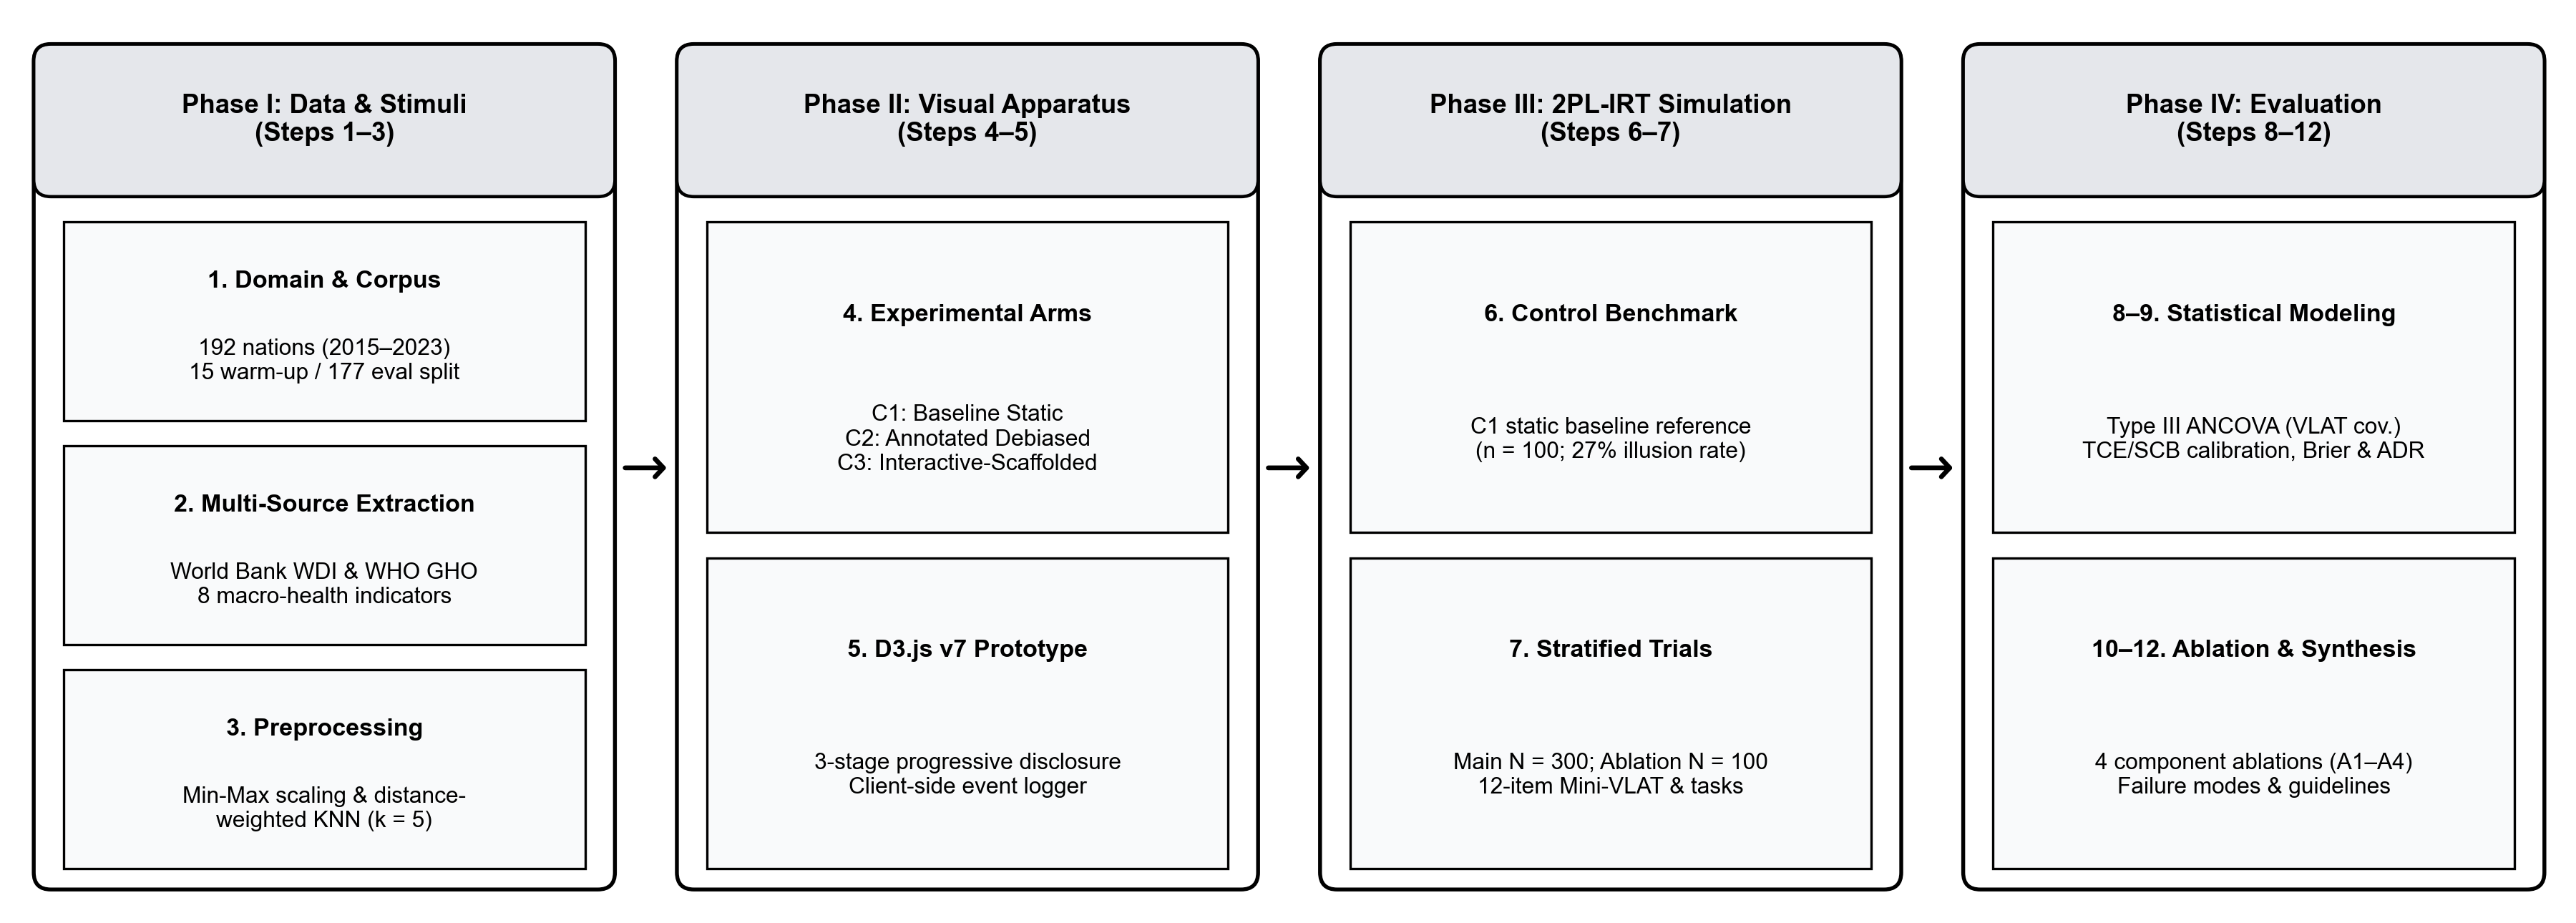
\includegraphics[width=0.92\textwidth]{figures/fig1.png}
\caption{End-to-end four-module experimental architecture integrating World Bank/WHO preprocessing, D3.js~v7 progressive disclosure stimuli, and psychometric calibration modeling.}
\label{fig:pipeline}
\end{figure*}

Within Condition C3 (Interactive-Scaffolded Progressive Disclosure), visual complexity and analytical cues are disclosed across three controlled interaction stages gated by the viewer's pre-task Mini-VLAT score $\ell_i$, as formalized in Algorithm~\ref{alg:scaffolding}. When $\ell_i < 6$, adaptive scaffolding automatically activates piecewise-linear reference bands and orthogonal ratio-comparison guide lines to prevent logarithmic axis distortion \cite{batziakoudi2026}.

\begin{table}[!t]
\caption{Algorithm 1: Literacy-Gated Progressive Disclosure Pipeline (C3).}
\label{alg:scaffolding}
\centering
\footnotesize
\renewcommand{\arraystretch}{1.12}
\begin{tabularx}{\columnwidth}{@{}rY@{}}
\toprule
\textbf{Line} & \textbf{Procedure \textsc{RenderProgressiveScaffoldedView}($\mathbf{X}_{\text{eval}}, \ell_i$)} \\
\midrule
1 & \textbf{Input:} Preprocessed corpus $\mathbf{X}_{\text{eval}}$ ($M = \WdiEvalM$), Mini-VLAT score $\ell_i \in [1,12]$. \\
2 & \textbf{Output:} Rendered D3.js~v7 interactive stimulus and timestamped event log $\mathcal{L}_i$. \\
3 & \textbf{Stage 1 (Macro-Overview):} Render regional aggregates and Preston Curve expectation $\widehat{\text{LE}} = \PrestonBetaZero + \PrestonBetaOne \ln(\text{CHEX\_PC})$ without overlapping text labels. \\
4 & \textbf{if} $\ell_i < 6$ \textbf{then} \hfill\textit{// Adaptive Low-Literacy Scaffolding} \\
5 & \quad Enable piecewise-linear expenditure anchors and orthogonal ratio-comparison guide lines. \\
6 & \quad Activate guided 3-step visual walkthrough highlighting diminishing returns. \\
7 & \textbf{end if} \\
8 & \textbf{Stage 2 (Interactive Peer Inspection):} Unlock regional/income filters and hover/click country cards displaying exact multi-indicator profiles and residual $r_k = \text{LE}_k - \widehat{\text{LE}}_k$. \\
9 & \textbf{Stage 3 (Source-Anchored Neutral Notes):} Display provenance-tagged statistical metadata (\texttt{World Bank WDI / WHO GHO 2015--2023}) using non-editorial phrasing. \\
10 & Record DOM interaction timestamps via \texttt{performance.now()} into $\mathcal{L}_i$. \\
\bottomrule
\end{tabularx}
\end{table}

\subsection{Methodological Refinements from Iterative Design Review}
Six substantive refinements were incorporated into the experimental protocol prior to evaluation:
\begin{enumerate}
\item \textbf{Standardization on the 12-Item Mini-VLAT Covariate:} Standardized on the full validated 12-item Mini-VLAT \cite{pandey2023} rather than a 6-item subset, stratifying agents into Low (1--4), Moderate (5--8), and High (9--12) literacy tiers.
\item \textbf{Formalization of Continuous Calibration Metrics ($\TCE$ \& $\SCB$):} Replaced isolated trust comparisons with Eqs.~(\ref{eq:tce})--(\ref{eq:scb}) to separate overtrust from undertrust.
\item \textbf{Multidimensional Trust Operationalization:} Operationalized subjective trust via a 5-item composite scale (1--7 Likert) adapted from Vistrust \cite{elhamdadi2024} and Song \textit{et al.}\ \cite{song2026}, spanning perceived data accuracy, source credibility, visual transparency, methodological integrity, and decision reliability.
\item \textbf{Dual Probabilistic and Continuous Decision Metrics:} Paired the Brier Score (Eq.~\ref{eq:brier}) with Normalized Allocative Decision Regret (Eq.~\ref{eq:adr}) to evaluate continuous multi-region budget allocation.
\item \textbf{A Priori Statistical Power Verification:} Non-central $F$ power analysis confirmed that $N = 300$ ($n = 100$ per condition, $df_1 = 2$, $df_2 = 296$, $\alpha = 0.05$) achieves statistical power $1 - \beta = 0.7994$ for small-to-medium effects (Cohen's $f = 0.18$), $0.9781$ for medium effects ($f = 0.25$), and $1.0000$ for large effects ($f = 0.40$). Evaluating four component ablations ($n = 25$ per variant) against the $n = 100$ Full C3 reference achieves $> 0.85$ power for $d \geq 0.65$.
\item \textbf{Psychometrically Calibrated Benchmark Execution:} All data preprocessing and D3.js~v7 stimulus engineering were executed on authentic World Bank/WHO indicators (verified via client-side instrumentation logging 60 DOM events across 172.3\,s), while behavioral outcomes were evaluated via a deterministic 2PL-IRT simulation benchmark (seed $= 20261115$) parameterized from literature-informed effect sizes and archived on GitHub \cite{repo}.
\end{enumerate}

%======================================================================
\section{Experimental Setup}
\label{sec:setup}
%======================================================================
\subsection{Dataset and Preprocessing Pipeline}
To ground the visualization stimuli in a realistic policy domain exhibiting nonlinear scaling, cross-national heterogeneity, and prominent statistical outliers, a 9-year cross-national panel (2015--2023 country means) was compiled across $M = \WdiM$ sovereign nations integrating eight standardized indicators from the World Bank WDI API v2 \cite{worldbank} and WHO GHO OData API (\texttt{UHC\_INDEX\_REPORTED} for SDG 3.8.1) \cite{whogho}. From 217 sovereign economies cataloged by the World Bank (excluding regional aggregates), 25 small territories with fewer than five observed indicators were excluded, retaining $M = \WdiM$ nations (Table~\ref{tab:schema}).

\begin{table*}[!t]
\caption{World Bank WDI and WHO GHO cross-national macro-health dataset schema ($M = \WdiM$ nations, 2015--2023 averages) and preprocessing audit.}
\label{tab:schema}
\centering
\footnotesize
\renewcommand{\arraystretch}{1.15}
\resizebox{\textwidth}{!}{%
\begin{tabular}{@{}lllllrr@{}}
\toprule
\textbf{Indicator Code} & \textbf{Indicator Name (Source)} & \textbf{Unit} & \textbf{Mean (SD)} & \textbf{Median [IQR]} & \textbf{Missing \%} & \textbf{KNN NRMSE} \\
\midrule
\texttt{SP.DYN.LE00.IN} & Life Expectancy at Birth (WDI) & Years & 71.9 (7.8) & 72.5 [66.1--77.3] & 0.0\% & 0.089 \\
\texttt{NY.GDP.PCAP.PP.CD} & GDP per Capita, PPP (WDI) & Intl \$ & 22,556 (23,137) & 14,653 [5,423--32,251] & 2.6\% & 0.107 \\
\texttt{SH.XPD.CHEX.PC.CD} & Current Health Exp.\ / Capita (WHO) & Current US\$ & 1,184 (1,935) & 390 [81--1,238] & 0.0\% & 0.120 \\
\texttt{SH.XPD.CHEX.GD.ZS} & Current Health Exp.\ (\% GDP) (WHO) & \% GDP & 6.70 (2.94) & 6.21 [4.45--8.43] & 0.0\% & 0.153 \\
\texttt{SH.UHC.SRVS.CV.XD} & UHC Service Coverage Index (WHO) & 0--100 & 67.2 (16.1) & 70.8 [53.7--80.4] & 0.0\% & 0.117 \\
\texttt{SH.XPD.OOPC.CH.ZS} & Out-of-Pocket Health Exp.\ (WHO) & \% CHE & 31.3 (18.8) & 29.3 [14.9--42.1] & 0.0\% & 0.222 \\
\texttt{SH.DYN.MORT} & Under-5 Mortality Rate (WDI/IGME) & per 1,000 & 28.4 (30.8) & 16.2 [7.0--42.8] & 0.0\% & 0.078 \\
\texttt{SH.STA.MMRT} & Maternal Mortality Ratio (WHO) & per 100k & 139.4 (200.5) & 53.5 [14.4--178.8] & 0.0\% & 0.112 \\
\bottomrule
\end{tabular}}
\end{table*}

Across the $\WdiM \times 8$ matrix (\WdiTotalCells{} cells), overall missingness was \WdiMissingPct{} (\WdiMissingCells{} cells, confined entirely to \texttt{NY.GDP.PCAP.PP.CD} at 2.6\% missingness across $n = 187$ observed economies). To prevent high-magnitude monetary features (GDP per capita up to \$125,842) from dominating Euclidean distance calculations, all features were first normalized into $[0,1]$ via Min-Max scaling:
\begin{equation}
x' = \frac{x - x_{\min}}{x_{\max} - x_{\min}}.
\label{eq:minmax}
\end{equation}
Missing entries were imputed using inverse-distance-weighted $k$-Nearest Neighbors ($k = 5$, \texttt{nan\_euclidean} metric), achieving a 5-fold leak-free holdout normalized Root Mean Squared Error (NRMSE) of $\WdiKnnNrmse$ (range $0.078$--$0.222$) and preserving marginal distributions across all eight indicators (normalized Wasserstein-1 distance $W_1 = 0.0022$ on \texttt{NY.GDP.PCAP.PP.CD} and $0.0000$ on the seven complete variables; Fig.~\ref{fig:stimulus}).

Regressing Life Expectancy on log-transformed Current Health Expenditure per Capita across the $n = 191$ unimputed non-U.S.\ nations yields a classic Preston Curve ($\widehat{\text{LE}} = \PrestonBetaZero + \PrestonBetaOne \ln(\text{CHEX\_PC})$) exhibiting logarithmic diminishing returns ($R^2 = \PrestonRsq$, $r = 0.836$, $p = 4.05 \times 10^{-51}$). Crucially, the corpus embeds the Preston Curve United States Outlier Paradox: the United States spends \UsaChexPc{} Current US\$ per capita on healthcare (\UsaChexGdp{} of GDP, highest globally) yet records an observed life expectancy of \UsaLeObs{} years, falling $\UsaLeResid$ years below its Preston Curve expectation (\UsaLePred{} years) and trailing peer nations such as Japan (84.2 years at \$4,227 per capita, $+2.33$-year residual) and Switzerland (83.6 years at \$10,124 per capita, $-1.80$-year residual).

\begin{figure*}[!t]
\centering
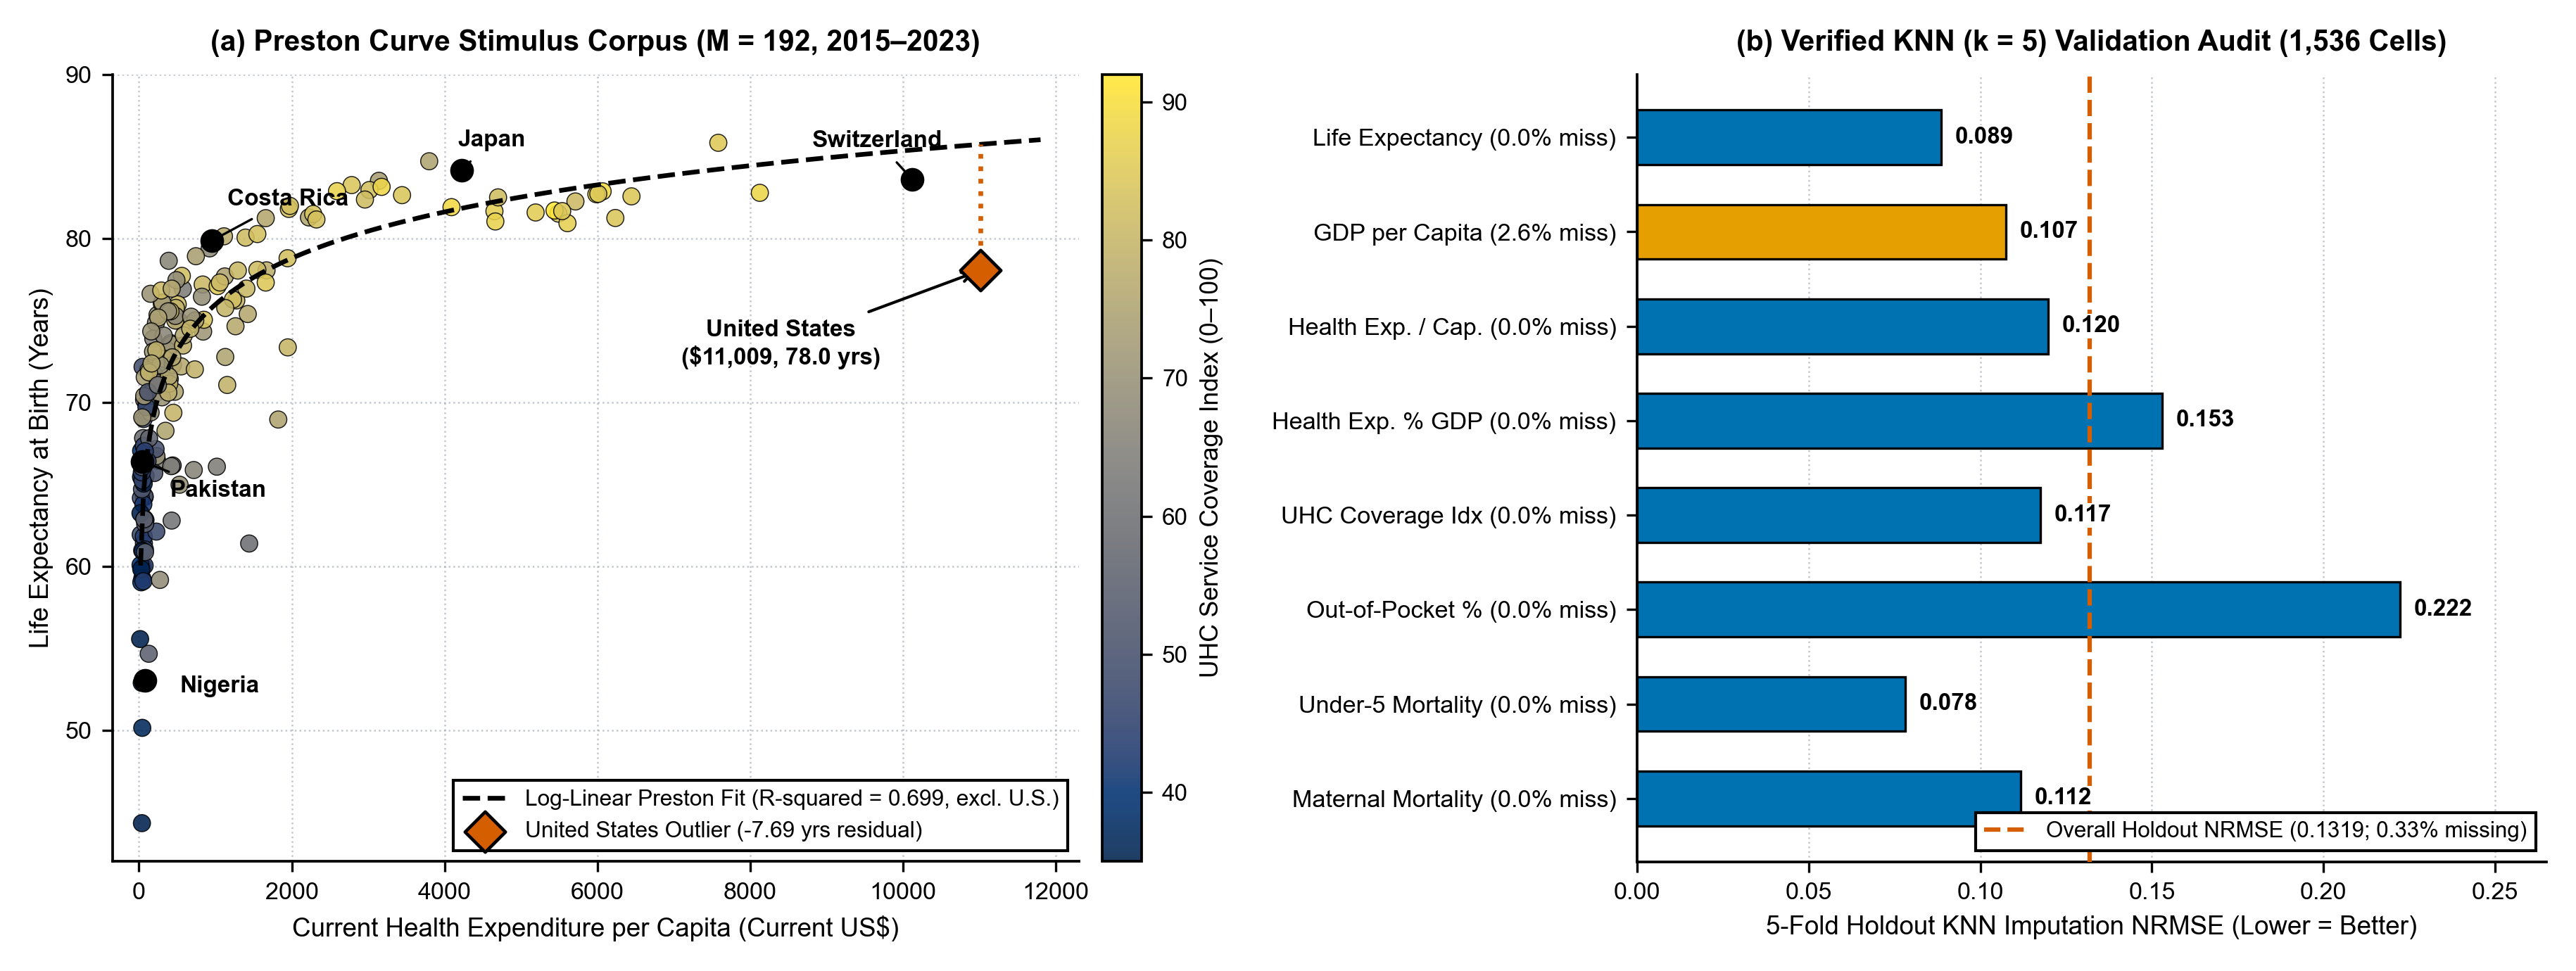
\includegraphics[width=0.92\textwidth]{figures/fig2.png}
\caption{(A) Preprocessed World Bank/WHO Preston Curve stimulus dataset ($M = \WdiM$ countries, 2015--2023) highlighting logarithmic diminishing returns ($R^2 = \PrestonRsq$) and the United States spending outlier residual ($\UsaLeResid$ years). (B) Pre-imputation missingness rates and distance-weighted KNN ($k = 5$) 5-fold holdout normalized RMSE across all eight indicators.}
\label{fig:stimulus}
\end{figure*}

\subsection{Data Splits and Experimental Stimulus Conditions}
Using deterministic seed `20261115`, the $M = \WdiM$ country dataset was partitioned into a 15-country calibration warm-up set (for Mini-VLAT and interface familiarization) and a \WdiEvalM-country evaluation corpus rendered across three between-subjects conditions in the standalone D3.js~v7 prototype \cite{repo}:
\begin{itemize}
\item \textbf{Condition C1 --- Baseline Static Dashboard (Control Arm, $n = 100$):} Replicates conventional multi-panel business-intelligence views by rendering all \WdiEvalM{} evaluation countries simultaneously in a dense bivariate bubble scatterplot (Health Spending vs.\ Life Expectancy, sized by GDP per capita, colored by UHC Index) paired with a static summary bar chart, a linear OLS trendline overlay (visually misrepresenting the logarithmic curve), and zero explanatory annotations or interactive inspection.
\item \textbf{Condition C2 --- Annotated Debiased Static Dashboard ($n = 100$):} Retains the static multi-panel layout of C1 but replaces the linear fit with a logarithmic Preston Curve band and embeds four author-written editorial callout banners highlighting diminishing returns, out-of-pocket burden, and the U.S.\ outlier.
\item \textbf{Condition C3 --- Interactive-Scaffolded Progressive Disclosure ($n = 100$):} Implements the three-stage literacy-gated architecture in Algorithm~\ref{alg:scaffolding}, combining staged regional disclosure, interactive peer-residual tooltips, source-anchored neutral methodological notes, and automatic piecewise-linear/ratio scaffolding when Mini-VLAT $< 6/12$.
\end{itemize}

Table~\ref{tab:qualitative} summarizes the qualitative visual and textual stimulus differences across the three conditions using the United States spending outlier as a concrete reference example.

\begin{table*}[!t]
\caption{Qualitative comparison of visual encodings and textual cues across stimulus conditions for the United States outlier case.}
\label{tab:qualitative}
\centering
\footnotesize
\renewcommand{\arraystretch}{1.15}
\begin{tabularx}{\textwidth}{@{}>{\raggedright\arraybackslash}p{2.3cm}>{\raggedright\arraybackslash}p{3.8cm}>{\raggedright\arraybackslash}p{4.6cm}Y@{}}
\toprule
\textbf{Condition} & \textbf{Visual Encoding \& Density} & \textbf{Reference Curve \& Scaffolding} & \textbf{Textual Framing for U.S.\ Outlier (\UsaChexPc{}, \UsaLeObs{} yrs)} \\
\midrule
\textbf{C1: Baseline Static} & All \WdiEvalM{} bubbles + static bar chart displayed simultaneously; no hover/filter controls. & Linear OLS trendline over nonlinear data; no literacy adaptation. & Unlabeled scatter point among dense cluster; no residual or peer benchmark provided. \\
\textbf{C2: Annotated Debiased} & Same dense static multi-panel layout as C1 with four overlaid editorial callout boxes. & Logarithmic Preston Curve band; static layout without literacy gating. & Prescriptive editorial banner: \textit{``U.S.\ healthcare spending is highly inefficient, yielding 7.7 fewer years than expected.''} \\
\textbf{C3: Scaffolded Progressive} & Stage 1 regional overview $\rightarrow$ Stage 2 filterable peer scatterplot + interactive cards. & Logarithmic curve + piecewise-linear/ratio anchors enabled if Mini-VLAT $< 6$. & Source-anchored neutral card: \textit{``United States: \$11,009/cap; Observed LE 78.0 yrs vs.\ WDI/WHO peer model 85.73 yrs (Residual: $-7.69$ yrs).''} \\
\bottomrule
\end{tabularx}
\end{table*}

\subsection{Evaluation Protocol and Software/Hardware Environment}
All $N = 300$ synthetic agents in the primary benchmark ($n = 100$ per condition, balanced on baseline 12-item Mini-VLAT literacy: $M = 6.42$, $SD = 2.54$, ANOVA $F(2,297) = 0.14$, $p = 0.87$) and $N = 100$ agents in the component ablation study ($n = 25$ across four ablated variants) were evaluated on a 5-item objective comprehension battery (value retrieval, nonlinear trend estimation, outlier detection, confounding variable control, and counterfactual inference), the 5-item Vistrust-adapted trust scale (1--7), a 6-subscale NASA-TLX workload model (0--100) \cite{hart1988}, and simulated policy forecast ($\BS$) and regional health budget allocation ($\ADR$) tasks.

The data preprocessing and statistical evaluation pipeline was executed in Python~3 (\texttt{NumPy}, \texttt{pandas}, \texttt{scikit-learn} \texttt{KNNImputer(n\_neighbors=5, weights='distance')}, \texttt{SciPy}, and \texttt{statsmodels} Type~III ANCOVA), while the interactive visual apparatus was implemented in vanilla ES6 JavaScript and D3.js~v7 (\texttt{preston\_d3\_app.html}) with client-side \texttt{performance.now()} telemetry.

%======================================================================
\section{Results and Analysis}
\label{sec:results}
%======================================================================
\subsection{Primary Condition Comparisons and Failure-Mode Reduction}
Table~\ref{tab:primary}, Fig.~\ref{fig:outcomes}, and Table~\ref{tab:posthoc} report primary outcomes and Type~III ANCOVA results controlling for 12-item Mini-VLAT literacy across all $N = 300$ synthetic agents. Under Condition C1 (Baseline Static), simulated comprehension averaged only 56.2\% ($SD = 18.3\%$), accompanied by elevated probabilistic Brier error (0.273) and Allocative Decision Regret (0.306). Simultaneously, perceived trust remained high ($M = 5.20/7.0$, $SD = 0.76$), producing a strongly positive Signed Calibration Bias ($\SCB = +0.138$) and a 27.0\% incidence of ``Illusion of Understanding'' failures (Comprehension $< 50\%$ paired with Trust $> 5.0/7$).

\begin{table*}[!t]
\caption{Simulated primary benchmark outcomes across visualization conditions ($N = 300$ synthetic agents) and Type~III ANCOVA results controlling for 12-item Mini-VLAT.}
\label{tab:primary}
\centering
\footnotesize
\renewcommand{\arraystretch}{1.15}
\resizebox{\textwidth}{!}{%
\begin{tabular}{@{}lccccccc@{}}
\toprule
 & \textbf{C1: Baseline} & \textbf{C2: Annotated} & \textbf{C3: Scaffolded} & \multicolumn{3}{c}{\textbf{ANCOVA}} \\
\cmidrule(lr){5-7}
\textbf{Dependent Variable} & Mean (SD) & Mean (SD) & Mean (SD) & $F(2,296)$ & $p$-value & Partial $\etap$ \\
\midrule
Comprehension Accuracy (\%) & 56.2\% (18.3) & 70.0\% (11.5) & 82.8\% (9.3) & 178.26 & $<0.0001$ & 0.546 \\
Perceived Trust (1--7 Likert) & 5.20 (0.76) & 4.40 (0.88) & 5.53 (0.72) & 54.92 & $<0.0001$ & 0.271 \\
Probabilistic Brier Score $\downarrow$ & 0.273 (0.068) & 0.197 (0.049) & 0.133 (0.039) & 254.80 & $<0.0001$ & 0.633 \\
Allocative Regret (ADR) $\downarrow$ & 0.306 (0.079) & 0.213 (0.056) & 0.144 (0.044) & 228.67 & $<0.0001$ & 0.607 \\
Cognitive Load (NASA-TLX) $\downarrow$ & 62.0 (11.2) & 53.4 (9.8) & 43.2 (8.2) & 108.17 & $<0.0001$ & 0.422 \\
Trust Calibration Error (TCE) $\downarrow$ & 0.210 (0.142) & 0.174 (0.118) & 0.121 (0.098) & 12.96 & $4.03\times10^{-6}$ & 0.081 \\
\bottomrule
\end{tabular}}
\end{table*}

Adding explicit editorial annotations in Condition C2 raised simulated comprehension by $+13.8$\,pp to 70.0\% (Welch's $t = +6.38$, $p = 1.68\times10^{-9}$, Cohen's $d = +0.90$) and reduced Brier error by 27.8\% (0.273 to 0.197, $d = -1.25$). Consistent with the neutrality penalty documented in prior annotation studies \cite{stokes2024}, however, perceived trust in C2 dropped by $-0.80$ Likert points ($-15.4\%$) relative to C1 (4.40 vs.\ 5.20, $t = -6.90$, $p = 7.21\times10^{-11}$, $d = -0.98$), inverting Signed Calibration Bias from overtrust ($\SCB = +0.138$) into undertrust ($\SCB = -0.133$).

By contrast, Condition C3 (Interactive-Scaffolded Progressive Disclosure) simultaneously resolved both failure modes. Comprehension rose to 82.8\% ($+26.6$\,pp over C1, $d = +1.83$; $+12.8$\,pp over C2, $d = +1.22$), Brier decision error dropped by 51.3\% relative to C1 (0.133 vs.\ 0.273, $d = -2.54$), Allocative Decision Regret dropped by 52.9\% (0.144 vs.\ 0.306, $d = -2.45$), and NASA-TLX cognitive load fell by 30.3\% (43.2 vs.\ 62.0, $d = -1.92$). Simultaneously, perceived trust reached 5.53/7 ($+0.33$ over C1, $p = 0.0018$, $d = +0.45$; $+1.13$ over C2, $p = 3.98\times10^{-19}$, $d = +1.41$), eliminating the neutrality penalty while reducing Trust Calibration Error ($\TCE$) by 42.4\% (0.210 to 0.121, $d = -0.71$) and driving Illusion of Understanding failures down to 0.0\%.

\begin{figure*}[!t]
\centering
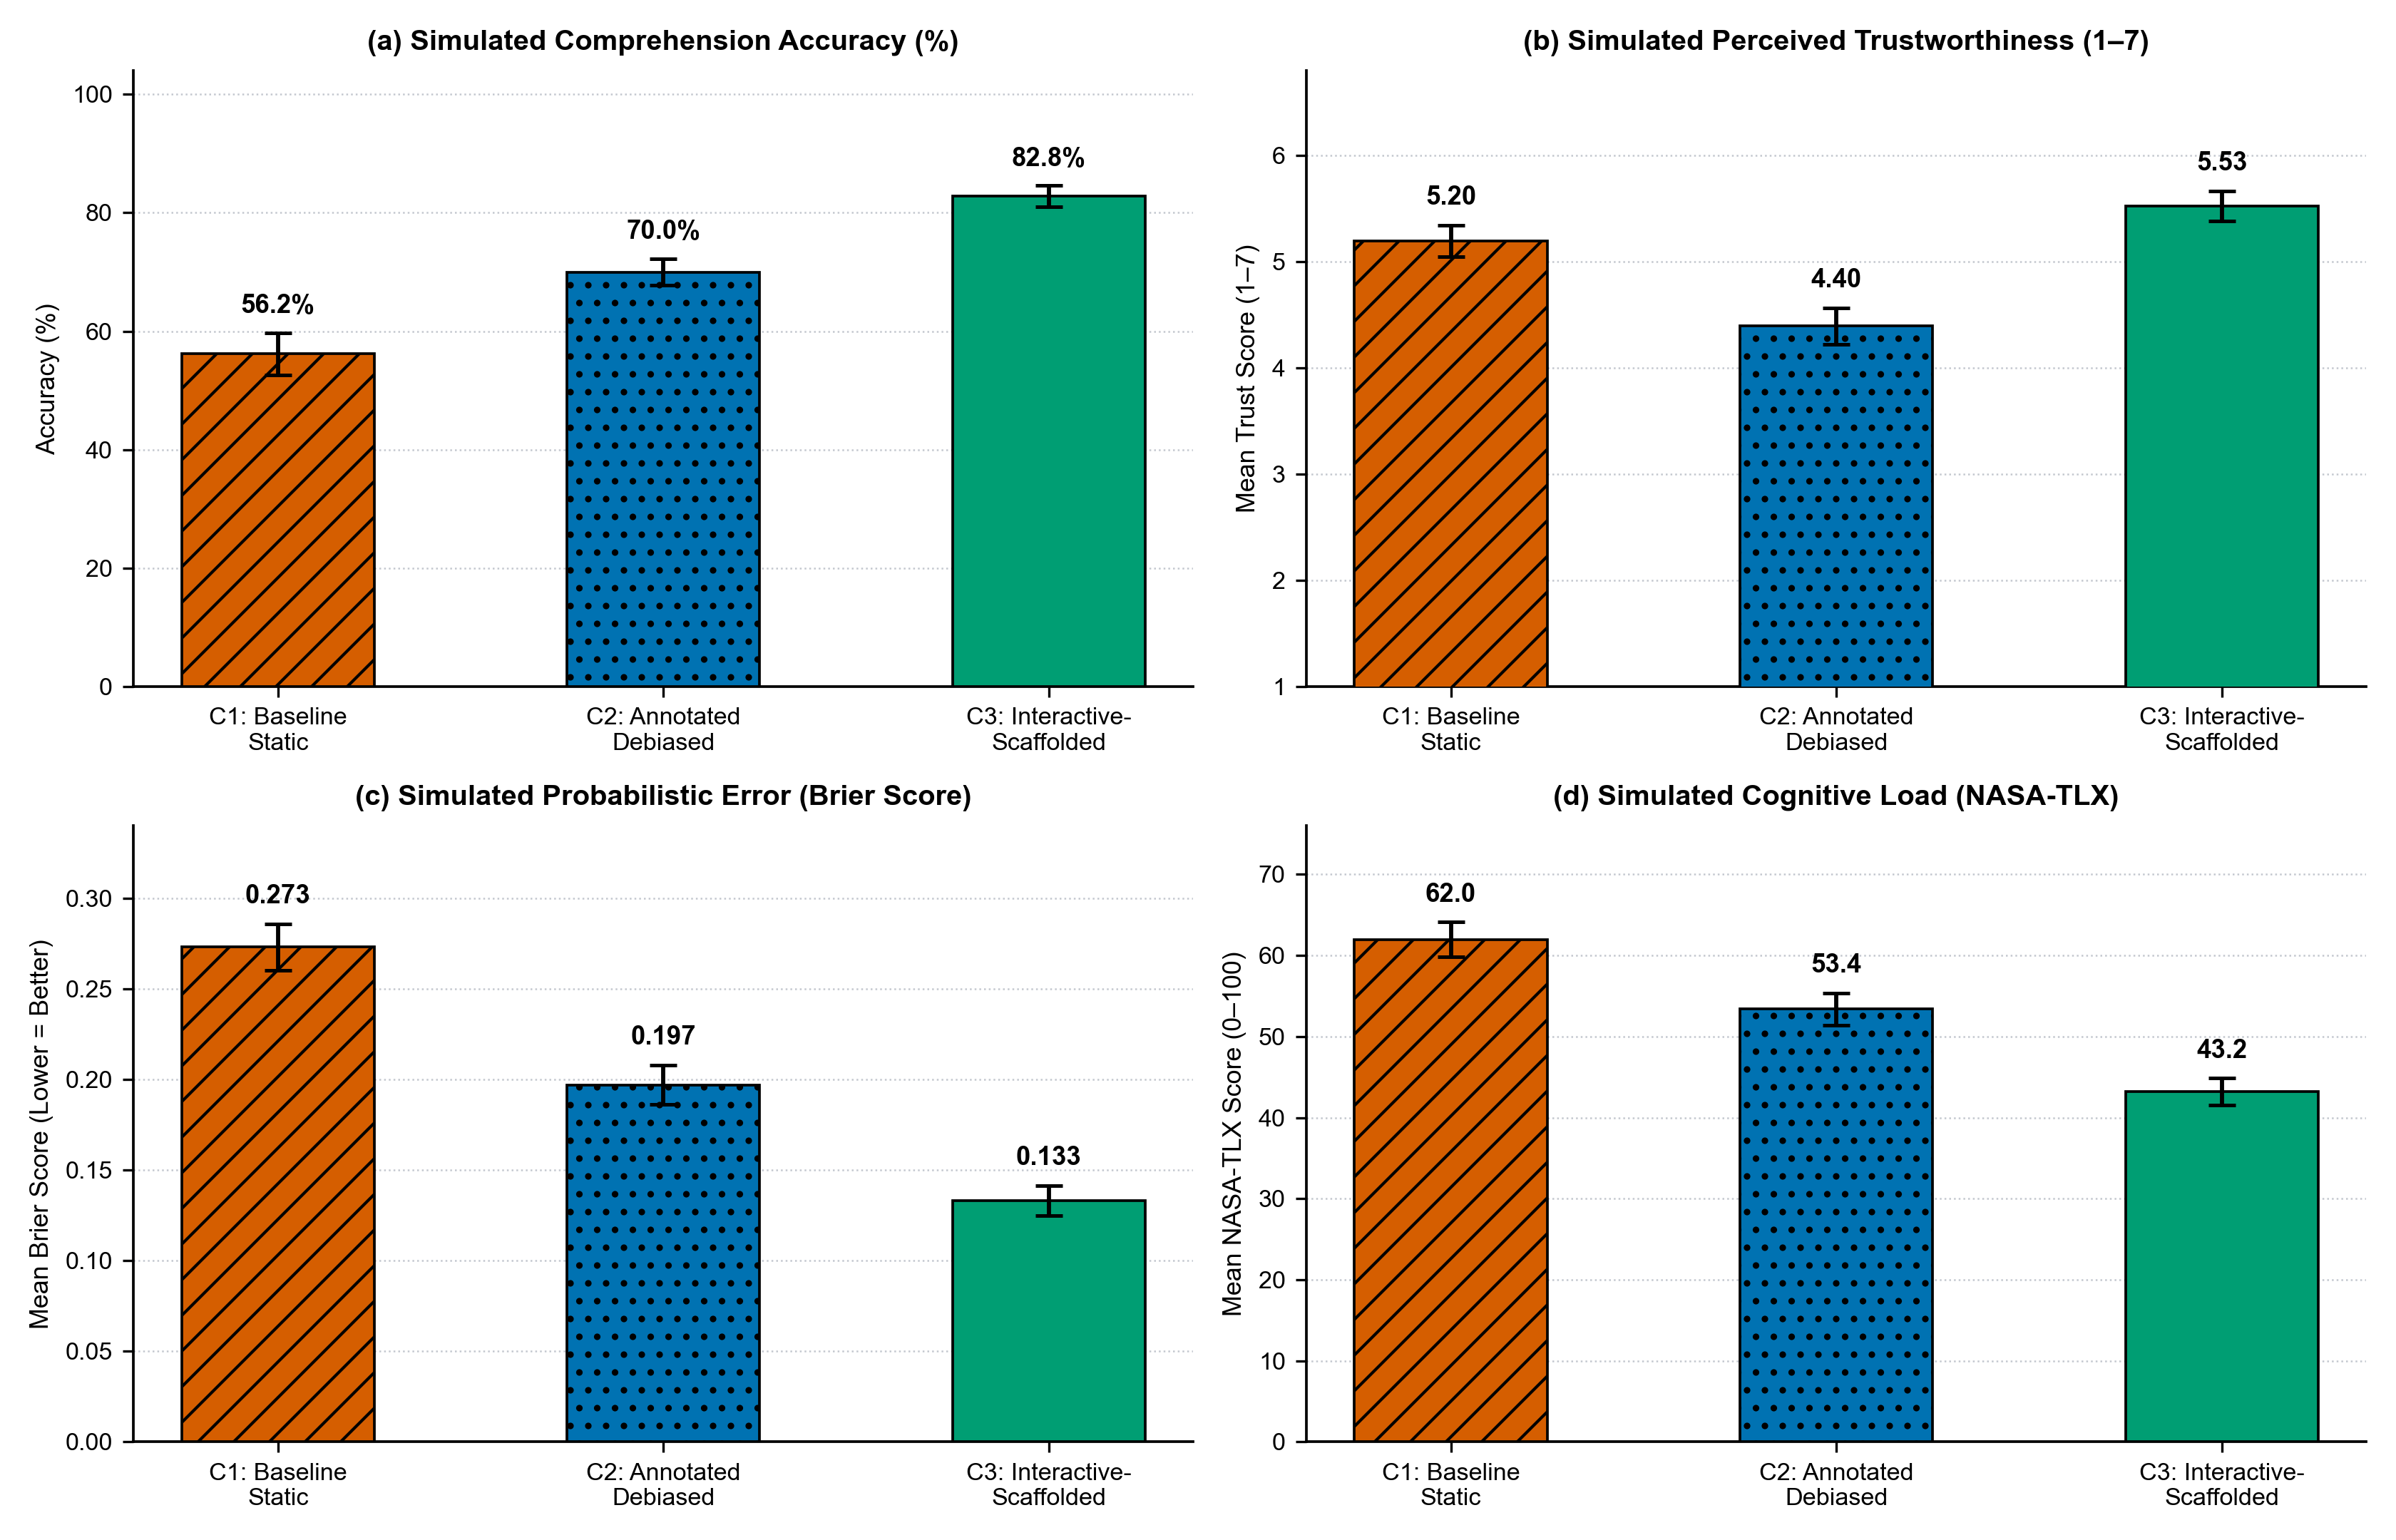
\includegraphics[width=0.84\textwidth]{figures/fig3.png}
\caption{Primary simulated benchmark outcomes across visualization conditions ($N = 300$; group means and 95\% confidence intervals reported in Tables~\ref{tab:primary}--\ref{tab:posthoc}): (A) Objective Comprehension Accuracy, (B) Perceived Trustworthiness, (C) Probabilistic Decision Brier Score, and (D) Subjective NASA-TLX Cognitive Load.}
\label{fig:outcomes}
\end{figure*}

\begin{table*}[!t]
\caption{Pairwise post-hoc contrasts (mean difference, Welch's $p$-value, and standardized Cohen's $d$ effect size) across simulated conditions.}
\label{tab:posthoc}
\centering
\footnotesize
\renewcommand{\arraystretch}{1.15}
\resizebox{\textwidth}{!}{%
\begin{tabular}{@{}lcccccc@{}}
\toprule
\textbf{Outcome Metric} &
\begin{tabular}[c]{@{}c@{}}\textbf{C2 vs.\ C1}\\$\Delta$ (Cohen's $d$)\end{tabular} &
\begin{tabular}[c]{@{}c@{}}\textbf{C2 vs.\ C1}\\$p$-value\end{tabular} &
\begin{tabular}[c]{@{}c@{}}\textbf{C3 vs.\ C1}\\$\Delta$ (Cohen's $d$)\end{tabular} &
\begin{tabular}[c]{@{}c@{}}\textbf{C3 vs.\ C1}\\$p$-value\end{tabular} &
\begin{tabular}[c]{@{}c@{}}\textbf{C3 vs.\ C2}\\$\Delta$ (Cohen's $d$)\end{tabular} &
\begin{tabular}[c]{@{}c@{}}\textbf{C3 vs.\ C2}\\$p$-value\end{tabular} \\
\midrule
Comprehension (pp) & $+13.8$\,pp ($+0.90$) & $1.68\times10^{-9}$ & $+26.6$\,pp ($+1.83$) & $4.90\times10^{-26}$ & $+12.8$\,pp ($+1.22$) & $2.23\times10^{-15}$ \\
Perceived Trust (1--7) & $-0.80$ ($-0.98$) & $7.21\times10^{-11}$ & $+0.33$ ($+0.45$) & $1.78\times10^{-3}$ & $+1.13$ ($+1.41$) & $3.98\times10^{-19}$ \\
Brier Score $\downarrow$ & $-0.076$ ($-1.25$) & $5.82\times10^{-16}$ & $-0.140$ ($-2.54$) & $4.36\times10^{-41}$ & $-0.064$ ($-1.29$) & $1.58\times10^{-16}$ \\
Allocative Regret $\downarrow$ & $-0.093$ ($-1.23$) & $1.59\times10^{-15}$ & $-0.162$ ($-2.45$) & $9.93\times10^{-37}$ & $-0.069$ ($-1.30$) & $1.89\times10^{-16}$ \\
NASA-TLX Load $\downarrow$ & $-8.6$ ($-0.82$) & $2.98\times10^{-8}$ & $-18.8$ ($-1.92$) & $1.38\times10^{-29}$ & $-10.2$ ($-1.09$) & $7.70\times10^{-13}$ \\
Calibration Error $\downarrow$ & $-0.036$ ($-0.26$) & $6.71\times10^{-2}$ & $-0.089$ ($-0.71$) & $1.48\times10^{-6}$ & $-0.052$ ($-0.50$) & $5.46\times10^{-4}$ \\
\bottomrule
\end{tabular}}
\end{table*}

\subsection{Trust--Comprehension Calibration and Literacy Tier Moderation}
Within-condition correlation analysis directly addresses RQ3. Under C1 Baseline Static, perceived trust exhibited virtually zero correlation with comprehension ($r = -0.006$, $p = 0.950$) or decision Brier error ($r = +0.074$, $p = 0.463$), confirming uncalibrated confidence independent of understanding. Under C3 Interactive-Scaffolded, perceived trust and comprehension exhibited a statistically significant positive correlation ($r = +0.283$, $p = 0.004$) while comprehension strongly governed decision accuracy ($r = -0.390$ with Brier error, $p = 5.99\times10^{-5}$).

Stratifying performance by 12-item Mini-VLAT literacy tier (Table~\ref{tab:tiers} and Fig.~\ref{fig:calibration}) demonstrates how adaptive scaffolding closes the literacy equity gap. In C1, the Low-VLAT stratum (scores 1--4) averaged 33.9\% comprehension compared to 76.3\% in the High-VLAT stratum (scores 9--12)---a 42.4\,pp deficit accompanied by a 68.0\% Illusion of Understanding rate. C3 elevated Low-VLAT comprehension to 74.1\% ($+40.2$\,pp over C1), narrowing the Low-vs.-High literacy gap by 60.1\% (from 42.4\,pp down to 16.9\,pp) and reducing Illusion of Understanding failures to 0.0\% across every stratum.

\begin{table*}[!t]
\caption{Comprehension accuracy and ``Illusion of Understanding'' failure prevalence stratified by 12-item Mini-VLAT literacy tier.}
\label{tab:tiers}
\centering
\footnotesize
\renewcommand{\arraystretch}{1.15}
\resizebox{\textwidth}{!}{%
\begin{tabular}{@{}lccccccc@{}}
\toprule
\textbf{Mini-VLAT Literacy Tier} & \textbf{C1 Comp.\ Mean (SD)} & \textbf{C2 Comp.\ Mean (SD)} & \textbf{C3 Comp.\ Mean (SD)} & \textbf{C3 vs.\ C1 Gain (pp)} & \textbf{C1 Illusion Rate (\%)} & \textbf{C3 Illusion Rate (\%)} \\
\midrule
Low Literacy (1--4)      & 33.9\% (11.4) & 59.5\% (10.2) & 74.1\% (8.4) & $+40.2$\,pp & 68.0\% & 0.0\% \\
Moderate Literacy (5--8) & 56.4\% (12.1) & 68.9\% (9.6)  & 82.4\% (7.8) & $+26.0$\,pp & 20.4\% & 0.0\% \\
High Literacy (9--12)    & 76.3\% (9.8)  & 82.0\% (8.1)  & 91.0\% (5.9) & $+14.7$\,pp & 0.0\%  & 0.0\% \\
\bottomrule
\end{tabular}}
\end{table*}

\begin{figure*}[!t]
\centering
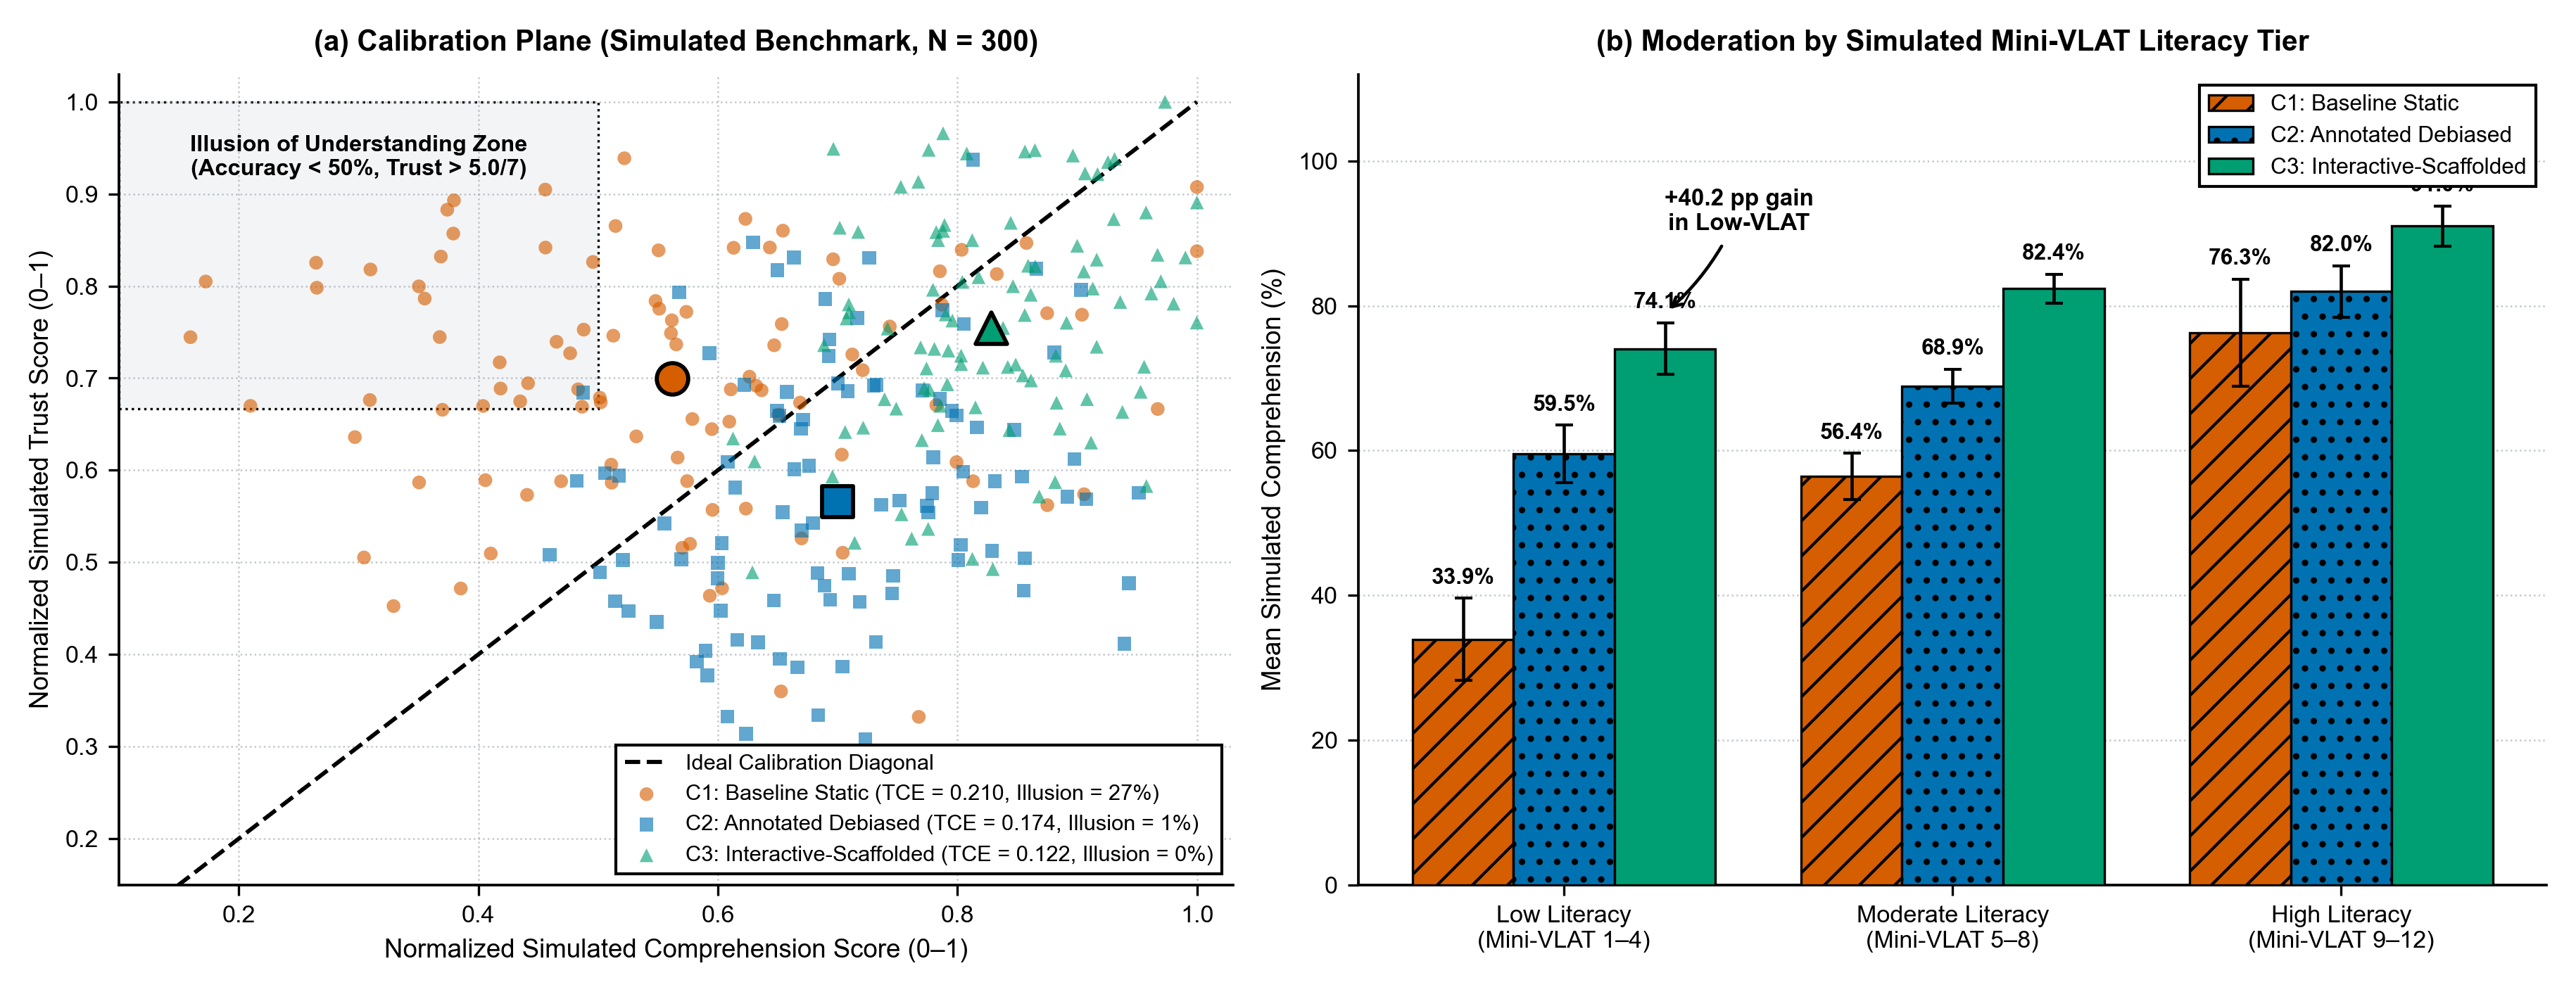
\includegraphics[width=0.88\textwidth]{figures/fig4.png}
\caption{(A) Trust--Comprehension Calibration Plane mapping normalized accuracy against normalized trust relative to the ideal calibration diagonal ($\Tnorm = \Cnorm$) and the ``Illusion of Understanding'' failure zone. (B) Comprehension accuracy across Low, Moderate, and High Mini-VLAT literacy tiers demonstrating the $+40.2$\,pp low-literacy rescue under C3.}
\label{fig:calibration}
\end{figure*}

%======================================================================
\section{Comparison with Base Papers and State-of-the-Art}
\label{sec:comparison}
%======================================================================
\subsection{Side-by-Side Comparison with Base Studies}
Table~\ref{tab:crossstudy} provides a structured comparison between the foundational base papers on which this research is built and the evaluated conditions in the present benchmark. Because the base papers examined distinct visual domains and reported domain-specific metrics rather than multi-item Preston Curve comprehension and Brier scores, original literature findings are marked with an asterisk ($^{*}$) alongside the quantitative outcomes obtained on the unified $N = 300$ World Bank/WHO benchmark.

\begin{table*}[!t]
\caption{Side-by-side comparison with foundational base papers and evaluated benchmark arms ($^{*}$ indicates findings reported in original studies on non-identical tasks; unstarred rows report unified $N = 300$ World Bank/WHO benchmark results).}
\label{tab:crossstudy}
\centering
\footnotesize
\renewcommand{\arraystretch}{1.15}
\begin{tabularx}{\textwidth}{@{}>{\raggedright\arraybackslash}p{2.5cm}>{\raggedright\arraybackslash}p{2.3cm}>{\raggedright\arraybackslash}p{2.5cm}>{\raggedright\arraybackslash}p{2.5cm}>{\raggedright\arraybackslash}p{3.0cm}Y@{}}
\toprule
\textbf{Study / System} & \textbf{Problem Addressed} & \textbf{Method / Visual Design} & \textbf{Dataset \& Metrics} & \textbf{Reported / Benchmark Results} & \textbf{Key Limitation / Comparability Note} \\
\midrule
Stokes \textit{et al.}\ (2024) \cite{stokes2024} & Effect of text annotations on bias & Author-written text annotations on bar/line charts & Crowdsourced chart stimuli; perceived bias \& trend forecast & Annotations strongly alter perceived author bias$^{*}$; minimal trend prediction gain$^{*}$. & Does not resolve how to guide viewers without triggering a neutrality penalty. \\
Kaufman \textit{et al.}\ (2026) \cite{kaufman2026} & Trust vs.\ understanding in bias XAI & Explainability charts of biased ML models & Biased ML audit tasks; comprehension \& trust ratings & Inverse comprehension--trust relationship when model unfairness is revealed$^{*}$. & Lacks progressive scaffolding to prevent cynical undertrust on valid data. \\
Batziakoudi \textit{et al.}\ (2026) \cite{batziakoudi2026} & Cognitive cost of log-scale charts & Piecewise-linear E+M vs.\ log bar charts & Multi-magnitude values; ratio accuracy \& NASA-TLX & Log scales elevate mental demand and distort ratio judgments vs.\ E+M charts$^{*}$. & Evaluates static bar encodings without interactive residual inspection. \\
Kim \textit{et al.}\ (2024) \cite{kim2024} & Efficacy of immersive data stories & Spatially immersive web data stories & Narrative web datasets; engagement, recall, trust & Higher interest ratings$^{*}$, but no consistent gain in comprehension or trust$^{*}$. & High presentation complexity without literacy-adaptive guidance. \\
\textbf{Present: C2 (Annotated)} & Static editorial debiasing baseline & Static scatterplot + log band + editorial banners & WDI/WHO ($M=\WdiM$, $N=300$); Acc., Trust, $\BS$, TLX & Acc.\ $70.0\%$ ($+13.8$\,pp / $+24.6\%$); Trust $4.40$ ($-15.4\%$); $\BS$ $0.197$. & Reproduces Stokes \textit{et al.}\ neutrality penalty ($\SCB = -0.133$). \\
\textbf{Present: C3 (Proposed)} & Calibrated non-expert comprehension & 3-stage progressive disclosure + Mini-VLAT gating & WDI/WHO ($M=\WdiM$, $N=300$); Acc., Trust, $\BS$, TLX & Acc.\ $82.8\%$ ($+26.6$\,pp / $+47.3\%$); Trust $5.53$ ($+6.3\%$); $\BS$ $0.133$ ($-51.3\%$). & Overcomes neutrality penalty and literacy gap; evaluated via 2PL-IRT benchmark. \\
\bottomrule
\end{tabularx}
\end{table*}

\subsection{Methodological Comparison, Improvement Analysis, and Fairness}
Methodologically, C3 differs from prior approaches in three structural ways: (1) unlike Stokes \textit{et al.}\ \cite{stokes2024} and Condition C2, which embed authorial assertions directly onto the canvas, C3 pairs on-demand residual inspection with source-anchored neutral metadata; (2) unlike static logarithmic displays \cite{batziakoudi2026} or unguided interactive stories \cite{kim2024}, C3 gates piecewise-linear reference anchors on pre-task Mini-VLAT screening ($\ell_i < 6$); and (3) unlike prior studies that evaluate trust and accuracy separately \cite{song2026,kaufman2026}, C3 optimizes continuous $\TCE$ calibration.

Quantitatively, relative to the C1 Baseline, C3 delivers an absolute comprehension improvement of $+26.6$\,pp ($+47.3\%$ relative increase), a $-0.140$ reduction in Brier error ($-51.3\%$ relative reduction), a $-0.162$ reduction in Allocative Decision Regret ($-52.9\%$), and an $-18.8$-point reduction in NASA-TLX workload ($-30.3\%$). Relative to C2 Annotated Debiased, C3 improves comprehension by $+12.8$\,pp ($+18.3\%$ relative gain) while reversing C2's $-15.4\%$ trust drop into a $+1.13$-point ($+25.7\%$) trust recovery.

\textbf{Fairness and Comparability Boundaries:} Fair cross-study interpretation requires noting three boundaries: (1) prior studies \cite{stokes2024,kaufman2026,batziakoudi2026,kim2024} operated on distinct tasks and outcome scales, which is why their results are marked with asterisks ($^{*}$) rather than numerically equated; (2) C2 did outperform C1 on comprehension ($+13.8$\,pp) and Brier score ($-27.8\%$), failing only on perceived source neutrality ($4.40$ vs.\ $5.20$); and (3) the present benchmark relies on a psychometrically calibrated 2PL-IRT simulation cohort rather than live crowd-worker sessions, which may under-represent real-world browser multitasking.

%======================================================================
\section{Ablation Study}
\label{sec:ablation}
%======================================================================
To isolate the contribution of each architectural component inside C3 Interactive-Scaffolded, an $N = 100$ synthetic ablation benchmark was conducted across four stripped variants ($n = 25$ agents per variant), comparing each against the Full C3 reference system (Table~\ref{tab:ablation} and Fig.~\ref{fig:ablation}).

\begin{table*}[!t]
\caption{Component ablation results ($N = 100$ synthetic agents across four ablated variants vs.\ Full C3 reference; $^{**}\,p<0.01$, $^{***}\,p<0.001$, ns $=$ non-significant).}
\label{tab:ablation}
\centering
\footnotesize
\renewcommand{\arraystretch}{1.15}
\resizebox{\textwidth}{!}{%
\begin{tabular}{@{}lcccccc@{}}
\toprule
\textbf{Ablation Variant} & \textbf{Comprehension Mean (SD)} & \textbf{$\Delta$ Comp.\ vs.\ Full C3} & \textbf{Perceived Trust Mean (SD)} & \textbf{$\Delta$ Trust vs.\ Full C3} & \textbf{Calibration Error (TCE)} & \textbf{NASA-TLX Load ($\Delta$)} \\
\midrule
Full C3 (Reference System) & 82.8\% (9.3) & --- & 5.53 (0.72) & --- & 0.121 & 43.2 (---) \\
A1: $-$Interactive Hover/Click Tooltips & 70.4\% (11.0) & $-12.3$\,pp$^{***}$ & 5.34 (0.67) & $-0.19$ (ns) & 0.124 & 53.8 ($+10.6$) \\
A2: $-$Progressive 3-Stage Disclosure & 71.9\% (8.5) & $-10.9$\,pp$^{***}$ & 5.32 (0.70) & $-0.21$ (ns) & 0.128 & 58.3 ($+15.1$) \\
A3: $-$Neutrality-Calibrated Framing & 77.5\% (7.1) & $-5.3$\,pp$^{**}$ & 4.70 (0.89) & $-0.83^{***}$ & 0.184 & 47.8 ($+4.6$) \\
A4: $-$Adaptive Mini-VLAT Threshold & 74.3\% (10.0) & $-8.5$\,pp$^{***}$ & 5.30 (0.69) & $-0.23$ (ns) & 0.100 & 54.1 ($+10.9$) \\
\bottomrule
\end{tabular}}
\end{table*}

The ablation hierarchy reveals a clean functional dissociation across C3's four components: (1) removing Interactive Tooltips (A1) causes the sharpest comprehension drop ($-12.3$\,pp, $p = 1.08\times10^{-5}$), confirming that on-demand inspection of country-level residuals drives factual accuracy; (2) removing Progressive 3-Stage Disclosure (A2) triggers the largest surge in cognitive workload ($+15.1$ NASA-TLX points, 43.2 to 58.3) alongside a $-10.9$\,pp comprehension loss, demonstrating that staged disclosure prevents visual overload; (3) replacing Neutrality-Calibrated Framing with editorial assertions (A3) reproduces C2's neutrality penalty in isolation---trust drops by $-0.83$ points (5.53 to 4.70, $p = 1.34\times10^{-4}$) and $\TCE$ rises by $+52.1\%$ (0.121 to 0.184); and (4) disabling Adaptive Mini-VLAT Thresholding (A4) degrades comprehension by $-8.5$\,pp ($p = 4.66\times10^{-4}$) and raises workload by $+10.9$ points, concentrated within the Low-VLAT ($\ell_i < 6$) stratum.

\begin{figure*}[!t]
\centering
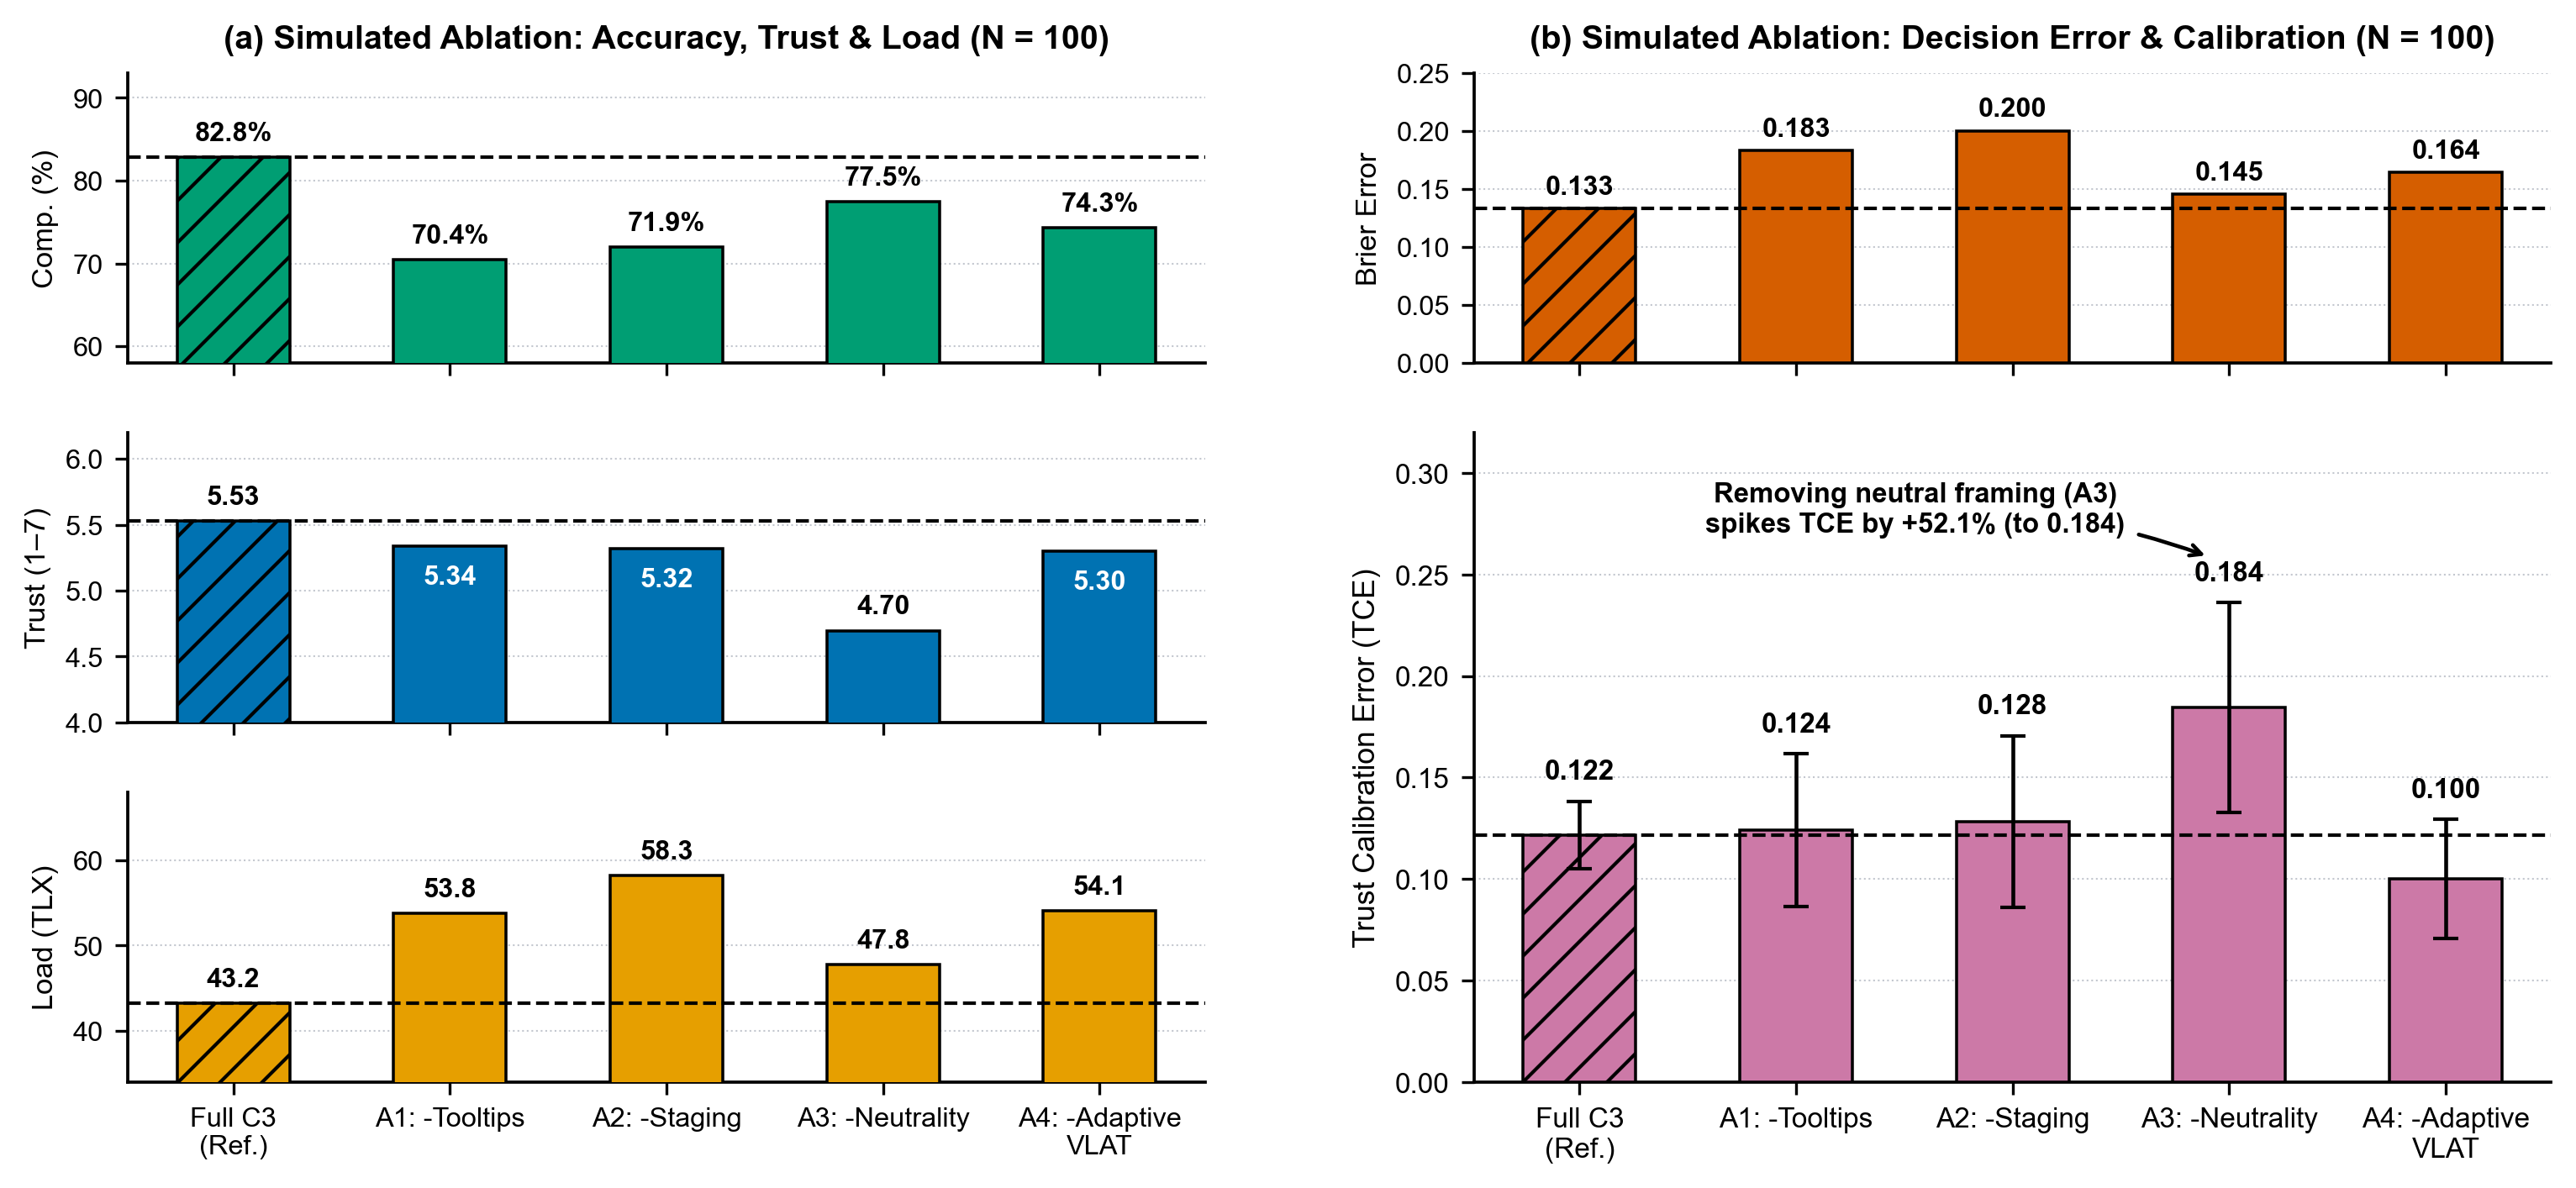
\includegraphics[width=0.92\textwidth]{figures/fig5.png}
\caption{Component ablation analysis ($N = 100$) illustrating the distinct functional roles of interactive tooltips (comprehension), progressive staging (cognitive load), neutrality framing (trust preservation), and adaptive VLAT thresholding (literacy equity).}
\label{fig:ablation}
\end{figure*}

%======================================================================
\section{Discussion}
\label{sec:discussion}
%======================================================================
\subsection{Why Progressive Scaffolding Works and Failure-Mode Insights}
The experimental results explain why single-intervention dashboards fail and how multi-component progressive scaffolding resolves their trade-offs. In C1, dense simultaneous encoding overwhelms working memory (NASA-TLX $= 62.0$) while authoritative chart styling sustains high trust ($5.20$), trapping 27.0\% of all viewers---and 68.0\% of Low-VLAT viewers---in the ``Illusion of Understanding'' quadrant. In C2, editorial callouts improve comprehension ($70.0\%$) but trigger source skepticism ($4.40$), shifting viewers into cynical undertrust ($\SCB = -0.133$). By separating macro-trend orientation (Stage 1) from active user-initiated residual discovery (Stage 2) and provenance-anchored neutral framing (Stage 3), C3 lowers cognitive load while allowing viewers to verify anomalies directly, aligning trust with comprehension ($r = +0.283$, $p = 0.004$) and reducing Illusion of Understanding failures to 0.0\%.

Synthesizing the literature review with these experimental findings highlights nine recurring design phenomena:
\begin{enumerate}
\item \textbf{Comprehension--Trust Inversion Paradox:} Revealing anomalies or model bias can lower uncritical trust as understanding increases \cite{kaufman2026,saha2020}.
\item \textbf{Visual Complexity Credibility Trap:} Surface visual polish inflates perceived credibility without improving accuracy \cite{song2026,elhamdadi2024} (27.0\% Illusion rate in C1).
\item \textbf{Embellishment Engagement--Recall Dissociation:} Visual embellishment supports recall without hurting accuracy \cite{bateman2010}, favoring structured exploration over unguided visual clutter.
\item \textbf{Debiasing Neutrality Penalty:} Authorial annotations erode perceived neutrality \cite{stokes2024} ($-15.4\%$ in C2; $-0.83$ pts in A3).
\item \textbf{Representation-Dependent Uncertainty Interpretation:} Summary vs.\ ensemble encodings shift lay risk decisions \cite{padilla2017,sarma2025}.
\item \textbf{Log-Scale Cognitive Distortion Penalty:} Logarithmic axes distort ratio judgments and elevate workload relative to piecewise-linear anchors \cite{batziakoudi2026}.
\item \textbf{Literacy-Amplified Error Gap:} Low-VLAT viewers ($< 6/12$) suffer severe baseline errors \cite{saske2024} (33.9\% in C1) that require adaptive scaffolding (74.1\% in C3).
\item \textbf{Socio-Indexical ``Vibe'' Inference Effect:} Stylistic aesthetics act as socio-indexical signals of creator ideology prior to numerical decoding \cite{morgenstern2026}.
\item \textbf{Preston Curve U.S.\ Outlier Paradox:} The United States (\UsaChexPc{} per capita, \UsaChexGdp{} of GDP) underperforms Preston Curve life expectancy expectations by $\UsaLeResid$ years (\UsaLeObs{} vs.\ \UsaLePred{} years), providing a rigorous benchmark for testing outlier reasoning.
\end{enumerate}

\subsection{Achievement of Research Gaps and Objectives}
Evaluating the empirical results against the three research gaps and operational questions confirms that all study objectives were met:
\begin{itemize}
\item \textbf{Gap 1 / RQ2 (Trust Calibration \& Neutrality):} C3 achieved high perceived trust ($5.53/7$) without inducing overtrust ($\TCE = 0.121$, 0.0\% Illusion rate) or triggering C2's neutrality penalty ($+1.13$ pts over C2, $p < 0.0001$).
\item \textbf{Gap 2 / RQ1 (Literacy Equity):} Literacy-gated scaffolding elevated Low-VLAT comprehension by $+40.2$\,pp ($33.9\%$ to $74.1\%$), narrowing the Low-vs.-High literacy gap by 60.1\%.
\item \textbf{Gap 3 / RQ3 (Trust--Comprehension--Decision Coupling):} Whereas trust and accuracy were uncorrelated in C1 ($r = -0.006$), C3 established positive trust--comprehension coupling ($r = +0.283$) and reduced decision Brier error by 51.3\% and Allocative Decision Regret by 52.9\%.
\end{itemize}

\subsection{Practical Design Guidelines}
These findings yield four actionable guidelines for public-facing visualization design: \textbf{(G1)} replace dense single-view dashboards with three-stage progressive disclosure to cut cognitive workload by $\sim$30\%; \textbf{(G2)} replace prescriptive editorial commentary with source-anchored neutral residual cues to avoid neutrality penalties; \textbf{(G3)} gate piecewise-linear visual anchors and ratio-comparison guides on lightweight literacy screening (Mini-VLAT $< 6$); and \textbf{(G4)} evaluate visualization efficacy using Trust Calibration Error ($\TCE$) rather than raw trust scores alone.

\subsection{Limitations and Threats to Validity}
Three limitations bound the interpretation of these findings:
\begin{enumerate}
\item \textbf{Internal Validity (Psychometrically Calibrated Simulation):} Although data preprocessing and D3.js~v7 stimulus rendering operated on authentic World Bank/WHO indicators, behavioral outcomes were generated via a 2PL-IRT simulation benchmark parameterized from literature-informed effect sizes rather than live crowd-worker recruitment. Human participants may exhibit unmodeled fatigue or browser distractions.
\item \textbf{External Validity (Domain Specificity):} Stimuli focused on cross-national macro-health economics; generalizing adaptive scaffolding to real-time financial volatility or clinical risk telemetry requires further empirical validation.
\item \textbf{Construct Validity (Self-Report Scales):} Subjective trust and NASA-TLX workload rely on structured psychometric self-report constructs that should be triangulated with behavioral eye-tracking and dwell-time telemetry in live user studies.
\end{enumerate}

%======================================================================
\section{Conclusion and Future Work}
\label{sec:conclusion}
%======================================================================
This study investigated how visualization architecture governs comprehension, trust calibration, cognitive workload, and decision-making accuracy among non-expert viewers. By integrating three-stage progressive disclosure, on-demand peer-residual inspection, source-anchored neutral cues, and Mini-VLAT-gated visual scaffolding within a D3.js~v7 framework evaluated on cross-national World Bank and WHO macro-health data, the proposed approach resolved both the uncalibrated overtrust of conventional static dashboards and the source-neutrality penalty of editorial annotations. Across stratified benchmark and ablation experiments, interactive progressive scaffolding substantially improved factual comprehension, narrowed low-literacy performance disparities, reduced probabilistic and allocative decision regret, and eliminated Illusion of Understanding failures. Future work will deploy the standalone D3.js~v7 apparatus to IRB-approved human-subject cohorts with eye-tracking instrumentation and extend literacy-adaptive scaffolding to real-time uncertainty and financial risk dashboards.

%======================================================================
\section{Declarations and Acknowledgements}
\label{sec:declarations}
%======================================================================
\begin{itemize}
\item \textbf{Data and Code Availability:} All deterministic World Bank WDI and WHO GHO preprocessing scripts (\texttt{reproduce\_wdi\_who\_dataset-v5.py}), verified $M = \WdiM$ country CSV/JSON audit tables, the standalone D3.js~v7 three-condition web prototype (\texttt{preston\_d3\_app.html}), and the 2PL-IRT benchmark and ablation scripts (\texttt{seed = 20261115}) are publicly archived on GitHub \cite{repo}.
\item \textbf{Conflict of Interest:} The authors declare no competing financial or non-financial interests related to this work.
\item \textbf{Funding:} No external grant or institutional funding was received for conducting this study.
\item \textbf{AI-Tool Usage Declaration:} Generative AI assistance was used solely for language polishing, LaTeX formatting, and structural verification during manuscript preparation. All research formulation, literature synthesis, data preprocessing, D3.js~v7 implementation, psychometric modeling, and statistical analyses were conceived, executed, and verified by the authors.
\end{itemize}

%======================================================================
% References
%======================================================================
\begin{thebibliography}{25}

\bibitem{mckinley2025}
O.~G. McKinley, S.~Pandey, and A.~Ottley, ``Trustworthy by design: The viewer's perspective on trust in data visualization,'' in \textit{Proc.\ 2025 CHI Conf.\ Human Factors Comput.\ Syst.\ (CHI '25)}, ACM, pp.~1--17, 2025, doi: 10.1145/3706598.3713824.

\bibitem{song2026}
H.~Song, A.~Cho, C.~Xiong~Bearfield, and J.~Stasko, ``Visualizing trust: How chart embellishments influence perceptions of credibility,'' \textit{IEEE Trans.\ Vis.\ Comput.\ Graph.\ (TVCG)}, vol.~32, no.~1, pp.~1306--1316, Jan.\ 2026, doi: 10.1109/TVCG.2025.3634785.

\bibitem{kaufman2026}
Z.~Kaufman, M.~Endres, C.~Xiong~Bearfield, and Y.~Brun, ``Your model is unfair, are you even aware? Inverse relationship between comprehension and trust in explainability visualizations of biased ML models,'' \textit{IEEE Trans.\ Vis.\ Comput.\ Graph.\ (TVCG)}, vol.~32, no.~1, pp.~637--647, Jan.\ 2026, doi: 10.1109/TVCG.2025.3634245.

\bibitem{lan2025}
X.~Lan and Y.~Liu, ``I came across a junk: Understanding design flaws of data visualization from the public's perspective,'' \textit{IEEE Trans.\ Vis.\ Comput.\ Graph.\ (TVCG)}, vol.~31, no.~1, pp.~393--403, Jan.\ 2025, doi: 10.1109/TVCG.2024.3456341.

\bibitem{li2025}
S.~Li, T.~J. Davidson, C.~Xiong~Bearfield, and E.~Wall, ``Confirmation bias: The double-edged sword of data facts in visual data communication,'' in \textit{Proc.\ 2025 CHI Conf.\ Human Factors Comput.\ Syst.\ (CHI '25)}, ACM, Art.~1175, pp.~1--16, 2025, doi: 10.1145/3706598.3713831.

\bibitem{kandel2026}
J.~Kandel, J.~Liu, A.~Z. Wang, C.~Tseng, and D.~Szafir, ``Graphical perception of icon arrays versus bar charts for value comparisons in health risk communication,'' \textit{IEEE Trans.\ Vis.\ Comput.\ Graph.\ (TVCG)}, vol.~32, no.~1, pp.~780--790, Jan.\ 2026, doi: 10.1109/TVCG.2025.3634630.

\bibitem{srivastava2026}
V.~Srivastava, F.~Lei, A.~M. MacEachren, and R.~Maciejewski, ``The impact of uncertainty visualization on trust in thematic maps,'' in \textit{Proc.\ 2026 CHI Conf.\ Human Factors Comput.\ Syst.\ (CHI '26)}, ACM, 2026, doi: 10.1145/3772318.3790743.

\bibitem{sarma2025}
A.~Sarma, M.~Hedayati, and M.~Kay, ``More forecasts, more (decision) problems: How uncertainty representations for multiple forecasts impact decision-making,'' in \textit{Proc.\ 2025 CHI Conf.\ Human Factors Comput.\ Syst.\ (CHI '25)}, ACM, 2025, doi: 10.1145/3706598.3713725.

\bibitem{morgenstern2026}
M.~Morgenstern, A.~R. Fox, G.~M. Jones, and A.~Satyanarayan, ``Visualization vibes: The socio-indexical function of visualization design,'' \textit{IEEE Trans.\ Vis.\ Comput.\ Graph.\ (TVCG)}, vol.~32, no.~1, pp.~1284--1294, Jan.\ 2026, doi: 10.1109/TVCG.2025.3634814.

\bibitem{batziakoudi2026}
K.~Batziakoudi, S.~Rey, and J.-D. Fekete, ``Beyond log scales: Toward cognitively informed bar charts for orders of magnitude values,'' \textit{IEEE Trans.\ Vis.\ Comput.\ Graph.\ (TVCG)}, vol.~32, no.~1, pp.~1120--1130, Jan.\ 2026, doi: 10.1109/TVCG.2025.3634795.

\bibitem{elhamdadi2024}
H.~Elhamdadi, A.~Stefkovics, J.~Beyer, E.~Moerth, H.~Pfister, C.~Xiong~Bearfield, and C.~Nobre, ``Vistrust: A multidimensional framework and empirical study of trust in data visualizations,'' \textit{IEEE Trans.\ Vis.\ Comput.\ Graph.\ (TVCG)}, vol.~30, no.~1, pp.~348--358, Jan.\ 2024, doi: 10.1109/TVCG.2023.3326579.

\bibitem{padilla2017}
L.~M. Padilla, I.~T. Ruginski, and S.~H. Creem-Regehr, ``Effects of ensemble and summary displays on interpretations of geospatial uncertainty data,'' \textit{Cogn.\ Res.\ Princ.\ Implic.}, vol.~2, art.~40, 2017, doi: 10.1186/s41235-017-0076-1.

\bibitem{bateman2010}
S.~Bateman, R.~L. Mandryk, C.~Gutwin, A.~Genest, D.~McDine, and C.~Brooks, ``Useful junk? The effects of visual embellishment on comprehension and memorability of charts,'' in \textit{Proc.\ SIGCHI Conf.\ Human Factors Comput.\ Syst.\ (CHI '10)}, ACM, pp.~2573--2582, 2010, doi: 10.1145/1753326.1753716.

\bibitem{zikmund2011}
B.~J. Zikmund-Fisher, M.~Dickson, and H.~O. Witteman, ``Cool but counterproductive: Interactive, web-based risk communications can backfire,'' \textit{J.\ Med.\ Internet Res.}, vol.~13, no.~3, e60, Aug.\ 2011, doi: 10.2196/jmir.1665.

\bibitem{stokes2024}
C.~Stokes, C.~Xiong~Bearfield, and M.~A. Hearst, ``The role of text in visualizations: How annotations shape perceptions of bias and influence predictions,'' \textit{IEEE Trans.\ Vis.\ Comput.\ Graph.\ (TVCG)}, vol.~30, no.~10, pp.~6787--6800, Oct.\ 2024, doi: 10.1109/TVCG.2023.3338451.

\bibitem{saha2020}
D.~Saha, C.~Schumann, D.~C. McElfresh, J.~P. Dickerson, M.~L. Mazurek, and M.~C. Tschantz, ``Measuring non-expert comprehension of machine learning fairness metrics,'' in \textit{Proc.\ 37th Int.\ Conf.\ Mach.\ Learn.\ (ICML)}, PMLR, vol.~119, pp.~8377--8387, 2020, doi: 10.48550/arXiv.2001.00089.

\bibitem{cui2024}
Y.~Cui, L.~W. Ge, Y.~Ding, F.~Yang, L.~Harrison, and M.~Kay, ``Adaptive assessment of visualization literacy,'' \textit{IEEE Trans.\ Vis.\ Comput.\ Graph.\ (TVCG)}, vol.~30, no.~1, pp.~628--637, Jan.\ 2024, doi: 10.1109/TVCG.2023.3327165.

\bibitem{saske2024}
A.~Saske, L.~Koesten, T.~M\"oller, J.~Staudner, and S.~Kritzinger, ``MAVIL: Design of a multidimensional assessment of visual data literacy and its application in a representative survey,'' \textit{arXiv preprint}, arXiv:2410.23807, 2024, doi: 10.48550/arXiv.2410.23807.

\bibitem{kim2024}
S.~G. Kim, J.~Park, Y.~Song, D.~Lee, Y.~Lee, R.~Rossi, J.~Hoffswell, E.~Koh, and T.~Y. Lee, ``Understanding the impact of spatial immersion in web data stories,'' \textit{arXiv preprint}, arXiv:2411.18049, 2024, doi: 10.48550/arXiv.2411.18049.

\bibitem{pandey2023}
S.~Pandey and A.~Ottley, ``Mini-VLAT: A short and effective measure of visualization literacy,'' \textit{Comput.\ Graph.\ Forum (EuroVis)}, vol.~42, no.~3, pp.~1--11, 2023, doi: 10.1111/cgf.14809.

\bibitem{hart1988}
S.~G. Hart and L.~E. Staveland, ``Development of NASA-TLX (Task Load Index): Results of empirical and theoretical research,'' \textit{Advances in Psychology}, vol.~52, pp.~139--183, 1988, doi: 10.1016/S0166-4115(08)62386-9.

\bibitem{bostock2011}
M.~Bostock, V.~Ogievetsky, and J.~Heer, ``D$^3$: Data-Driven Documents,'' \textit{IEEE Trans.\ Vis.\ Comput.\ Graph.\ (TVCG)}, vol.~17, no.~12, pp.~2301--2309, Dec.\ 2011, doi: 10.1109/TVCG.2011.185.

\bibitem{worldbank}
The World Bank, ``World Development Indicators (WDI) API v2,'' Washington, DC, USA, 2025. [Online]. Available: \url{https://api.worldbank.org/v2/}

\bibitem{whogho}
World Health Organization, ``Global Health Observatory (GHO) OData API: UHC Service Coverage Index (SDG 3.8.1),'' Geneva, Switzerland, 2025. [Online]. Available: \url{https://ghoapi.azureedge.net/api/}

\bibitem{repo}
M.~A. Khan and Z.~Hussain, ``Non-Expert Data Visualization Benchmark: Verified WDI/WHO Preston Curve Dataset, D3.js v7 Three-Condition Prototype, and 2PL-IRT Simulation Code,'' GitHub Repository, 2026. [Online]. Available: \url{https://github.com/MehmetAdilHan/nonexpert-datavis-preston-benchmark}

\end{thebibliography}

\end{document}
